\documentclass[
    % twoside,
    a4paper,
    11pt,
    footinclude,
    % 12pt,
    DIV=11,
    english,
]{scrreprt}
\usepackage{scrhack} % NOTE: fix some KOMA warnigns
\usepackage[english]{babel}
\usepackage[utf8]{inputenc}
\usepackage[T1]{fontenc}



%% adapt for printing
\usepackage[
    a4paper,
    pdftex,
    % inner=30mm,
    % outer=30mm,
    % vmargin=30mm,
    % bindingoffset=0mm
]{geometry}

%% acronyms and glossary
\usepackage[
    single=true,
    sort=true,
    only-used=true
]{acro}

\setlength{\marginparwidth}{2cm}

%% comments for reviews
\usepackage{amssymb}% http://ctan.org/pkg/amssymb
\usepackage{pifont}% http://ctan.org/pkg/pifont

% PDF inclusion
\usepackage{pdflscape}
\usepackage[final]{pdfpages}

%% figures, diagrams, and plots
\usepackage{graphicx}
\usepackage{tikz}
\usepackage{pgfplots}
\usepackage{tabulary}
\usepackage{svg}
\usepackage{amsmath}

%% Subfigure for ordering multiple pictures in one figure scope
\usepackage{subfigure}

%% Figure placement
\usepackage{float} % use H option to force placement

%% used for bytefields
%\usepackage{bytefield}
%\usepackage{rotating}

\pgfplotsset{compat=newest}
\pgfplotsset{compat=1.9}
\usepgfplotslibrary{colorbrewer}

%% tables
\usepackage{booktabs}
\usepackage{tabularx}

%% units & Symbols
\usepackage{siunitx}
%\usepackage{textcomp} % Fix undefined symbols warnings for gensymb, see https://latex.org/forum/viewtopic.php?f=4&t=3364#p13124
%\usepackage{gensymb}

%% unifying quote marks when using different languages
%% NOTE: Fixes warning concerning polyglossia when including biblatex
\usepackage{csquotes}

%% bibliography
\usepackage[]{biblatex}
\addbibresource{bibliography.bib}

%% head- and footlines
\usepackage{scrlayer-scrpage}
\setkomafont{pagehead}{\normalfont\small\sffamily}
\setkomafont{pagefoot}{\small}
\setkomafont{pagenumber}{\normalfont\bfseries}

\usepackage{xcolor}
\newcommand{\blueconsolas}[1]{{\color{blue}\texttt{#1}}}
\newcommand{\yellowconsolas}[1]{{\color{orange}\texttt{#1}}}

\automark[chapter]{chapter}
%\automark[section]{section}

\ihead{}
\chead{}
\ohead{\headmark}
\ifoot*{}
\cfoot*{}
\ofoot*{\pagemark}

% special chapter mark
\renewcommand{\chaptermark}[1]{%
    \markboth{%
        \MakeUppercase{%
            \chapapp%
        }%
        \thechapter%
        $\bigl{|}$~%
        \textcolor{black}{%
            \MakeUppercase{%
                % \so{%
                    #1%
                % }%
            }%
        }%
    } {%
        \textcolor{black}{%
            \MakeUppercase{%
                % \so{%
                    #1%
                % }%
            }%
        }%
        $\bigl{|}$~%
        \MakeUppercase{%
            \chapapp%
        }%
        \thechapter%
    }%
}

% no indent at start of paragraphs
\parindent 0pt

% disable extra space after colon
\frenchspacing

%% hyperref
\usepackage{hyperref}
\hypersetup{
    hidelinks,
    breaklinks=true,
    pdfpagemode=UseNone,
    pageanchor=true,
    pdfpagemode=UseOutlines,
    plainpages=false,
    bookmarksnumbered=true,
}

\usepackage{graphicx}
\begin{document}
\pagestyle{plain}%
\pagenumbering{roman}

\begin{titlepage}
    \begin{figure}[!tbp]
        \centering
        \begin{minipage}[b]{0.55\linewidth}
            
\includegraphics[height=2cm]{pictures/HTWG_logo.png}
        \end{minipage}%
        \hfill%
        \begin{minipage}[b]{0.4\linewidth}
            \hfill%
            %
\includegraphics[height=2cm]{pictures/HTWG_logo.png}
        \end{minipage}%
    \end{figure}
    \centering
    {\scshape\Large HTWG - Hochschule für Technik, Wirtschaft und Gestaltung \par}
    \vspace{1cm}
    {\scshape\LARGE Masterprojektarbeit\par}
    \vspace{1.5cm}
    {\huge\bfseries User Guide UWB GUI\par}
    \vspace{2cm}
    {\Large Positionsbestimmung mittels Ultrabreitband \par}
    \vfill
    erstellt von\par
    Tom \textsc{Herter}\par
    EIM 3\par
    Mtr. 306971\par
    \&\par
    Sebastian \textsc{Krebs}\par
    EIM 3\par
    Mtr. 298229\par
    \vfill
    betreut durch\par
    Prof.\ Dr.~\textsc{Knievel}
    \vfill
% Bottom of the page
	{\large Konstanz, \today\par}
\end{titlepage}



%\cleardoublepage%
%\begingroup
    \let\clearpage\relax            % disable \clearpage
    \let\cleardoublepage\relax      % disable \cleardoublepage

    \chapter*{Zusammenfassung}
    \pdfbookmark[1]{Zusammenfassung}{Zusammenfassung}
    \fontsize{10}{12}\selectfont

    XXX
    % back of abstract page
    \vfill
    \newpage
    \thispagestyle{empty}
    ~\vfill
\endgroup           % enables \clearpage and \cleardoublepage again


%\cleardoublepage%
%\begingroup
    \let\clearpage\relax        % disable \clearpage
    \let\cleardoublepage\relax  % disable \cleardoublepage

    \pdfbookmark[1]{Eidesstattliche Erklärung}{Eidesstattliche Erklaerung}
    \chapter*{Eidesstattliche Erklärung}

    Ich erkläre hiermit an Eides statt, dass ich die vorliegende Arbeit selbständig verfasst
    und dabei keine anderen als die angegebenen Hilfsmittel benutzt habe.
    Sämtliche Stellen der Arbeit, die im Wortlaut oder dem Sinn nach Publikationen
    oder Vorträgen anderer Autoren entnommen sind, habe ich als solche kenntlich gemacht.
    Die Arbeit wurde bisher weder gesamt noch in Teilen einer anderen Prüfungsbehörde
    vorgelegt und auch noch nicht veröffentlicht.\par
    \vspace{2cm}

    \begin{minipage}[h]{0.4\linewidth}
        \begin{center}
            Karlsruhe, den \today\par
            \dotfill\\
            (Ort, Datum)
            \vspace*{2.5mm}
        \end{center}
    \end{minipage}%
    \hfill%
    \begin{minipage}[h]{0.5\linewidth}
        \begin{center}
            \vspace*{5.5mm}
            \dotfill\\
            (Unterschrift)
            \vspace*{2.5mm}
        \end{center}
    \end{minipage}%

    \vfill
    % Yardeye Disclaimer
    Die vorliegende Arbeit stellt mein persönliches Arbeitsergebnis dar und ist kein offizielles Dokument der Yardeye GmbH.

    % back of acknowledgement page
    \vfill
    \newpage
    \thispagestyle{empty}
    \vfill

\endgroup   % enable \clearpage and \cleardoublepage again


%\cleardoublepage%

\tableofcontents%
\pagebreak%

\setcounter{section}{0}
\pagestyle{headings}%
\pagenumbering{arabic}%
\setcounter{tocdepth}{1}
\setcounter{secnumdepth}{2} % default value for 'report' class is "2"

\chapter{Introduction}

\section{Description}

This software guide is designed to explain the concept of the firmware running on the UWB tag and all the UWB anchor devices. 
The goal is to give a understanding what classes and files are used and how the interoperate together. 
Additionally to this guide a fill Doxygen documentation will be provided. 

\section{Naming Conventions}
Within this Software Guide detailing the Time-of-Flight (TOF) function, it's important to note that the terms "initiator" and "tag" are used interchangeably. 
Both refer to the UWB (Ultra-Wideband) device responsible for initiating the TOF measurement by transmitting a UWB request to the relevant devices in its vicinity.

These devices can also be alternatively referred to as "anchor", "responder" or "landmark". This nomenclature is employed because these devices play the pivotal role of responding to the UWB request and guiding the initiator in computing the distance between them. The interchangeable use of these terms is intended to provide clarity and flexibility in describing the dynamic roles these devices undertake in the TOF measurement process.

\section{Basic functionality and setup}
The primary function of this setup revolves around the estimation of tag positions within a predefined coordinate space. 
This estimation is achieved by leveraging the distances between the tag and various anchors strategically placed within the room. 
To facilitate a clearer grasp of the setup's workings, an illustrative sketch featuring example coordinates can be found in Figure \ref{fig:setup_sketch}.
\vspace{4pt}
\newline
In this setup, the anchors are situated throughout the room in a deliberate yet arbitrary manner, each possessing known coordinates. 
The key to this system's functionality lies in the tag device's ability to discern the positions of these anchors. 
With this information, the tag can deduce its own location in all the X, Y and Z directions by gauging the distances to all the anchors.
\vspace{4pt}
\newline
In Figure \ref{fig:setup_sketch}, these distances are visually represented and labeled as d\_1 to d\_5. 
The critical aspect of this process is that it enables the tag device to employ an Extended Kalman Filter (EKF) for the purpose of position estimation. 
This filter algorithm plays a pivotal role in refining and enhancing the accuracy of the tag's estimated position within the coordinate space and is further discussed in chapter \ref{chap:EKF_Handling}. 

\begin{figure}[!hbt]
	\centering
	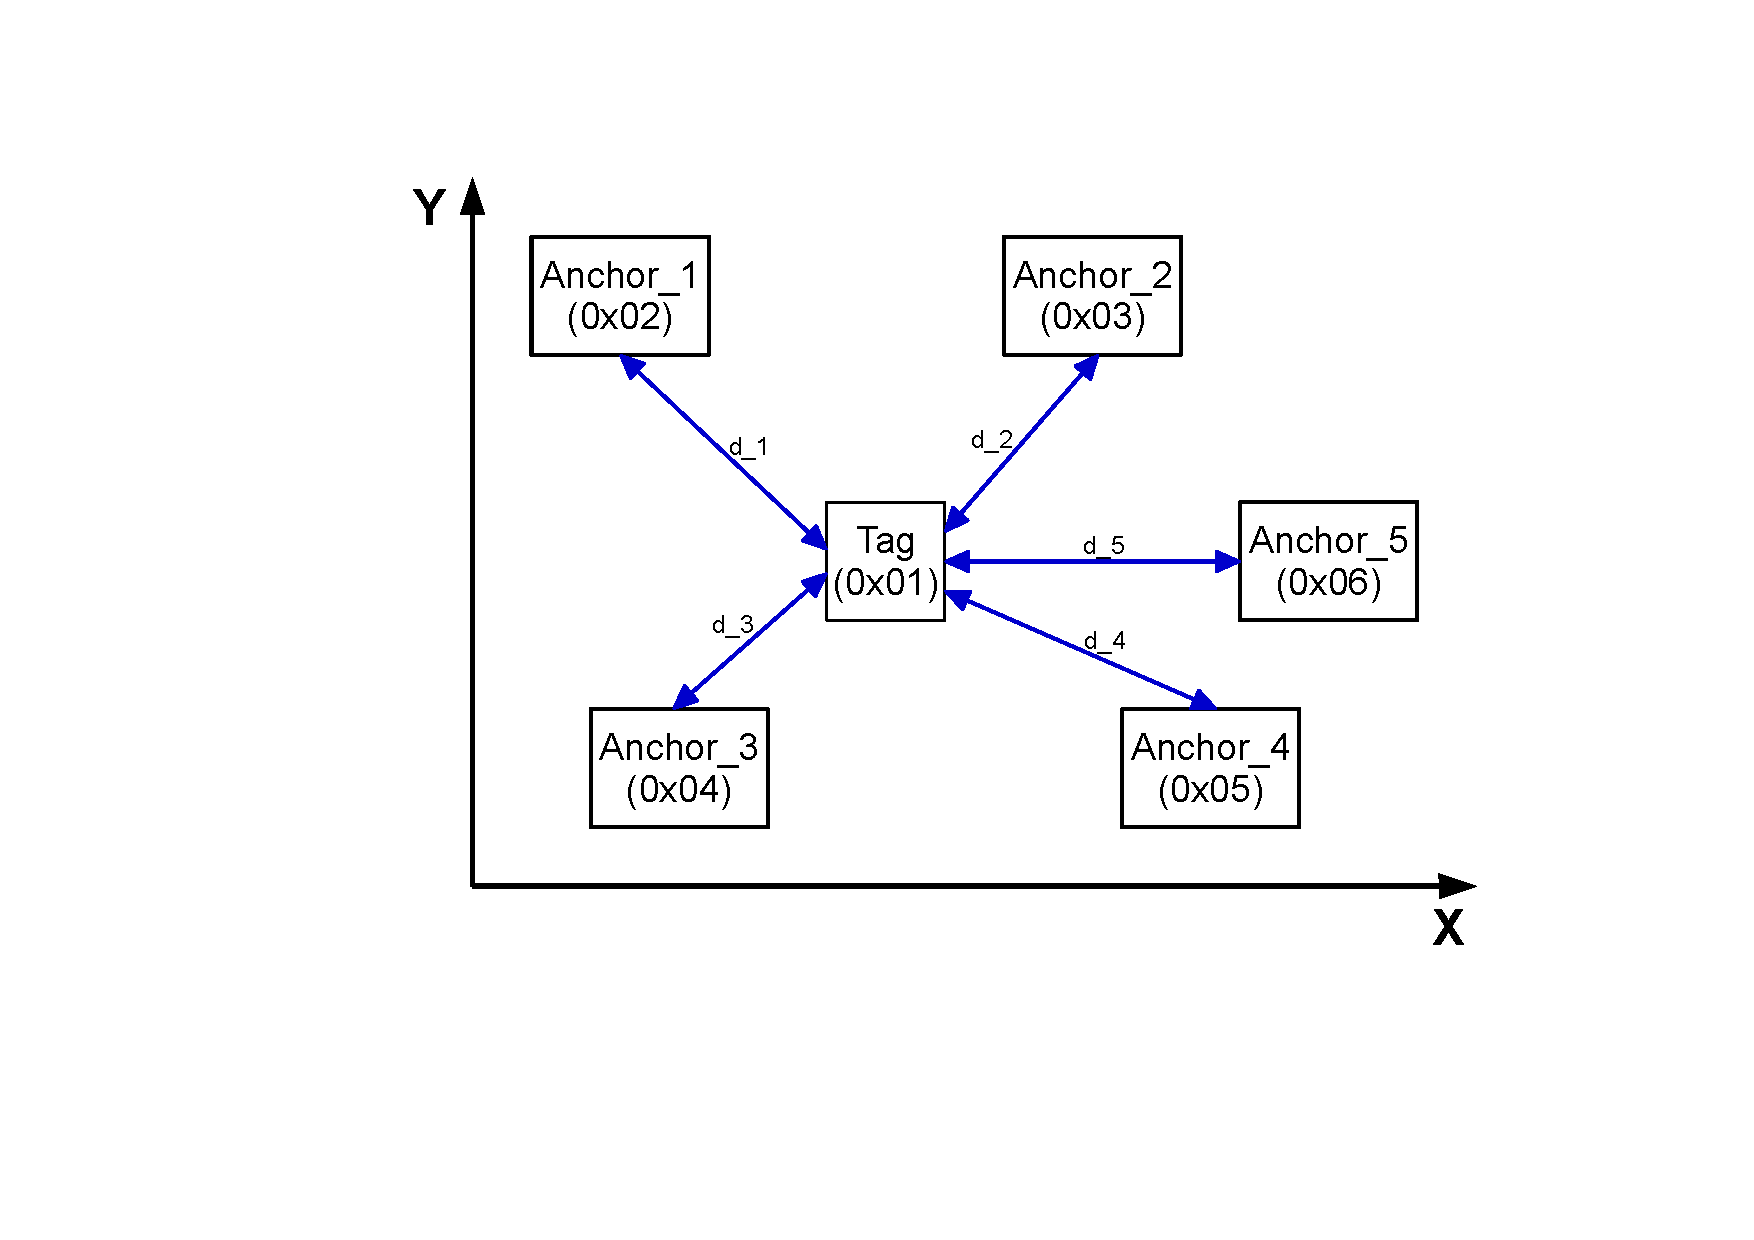
\includegraphics[width=0.6\textwidth]{pictures/Complete_Setup.pdf}
	\caption{Sketch of the complete setup.}
	\label{fig:setup_sketch}
\end{figure}

\section{Flow of Information}

In Figure \ref{fig:information_flow} the information flow of the entire system is pictured. 
The most important component are the UWB ranging messages exchanged between the Tag and every Anchor that are ultimately used to estimate the Tag's position. 
With every sent UWB message from the Tag to an Anchor the channel parameters are extracted and transmitted via WiFi to an MQTT-Server. 
The UWB Tag itself also transmits its coordinates over MQTT to a different topic. 
The MQTT mechanics are further discussed in \ref{chap:MQTT_Handling}. 
\vspace{4pt}
\newline
The configuration of the Tag, meaning putting in the coordinate of each anchor to the EEPROM, is executed via Bluetooth by a Bluetooth-Capable device running the configuration software. 
Additionally the Tag sends its position via Bluetooth where the configuration software has the ability to display it in a 2D plot in real time. 
Bluetooth Handling techniques are further elaborated in \ref{chap:Bluetooth_Handling}. 

\begin{figure}[!hbt]
	\centering
	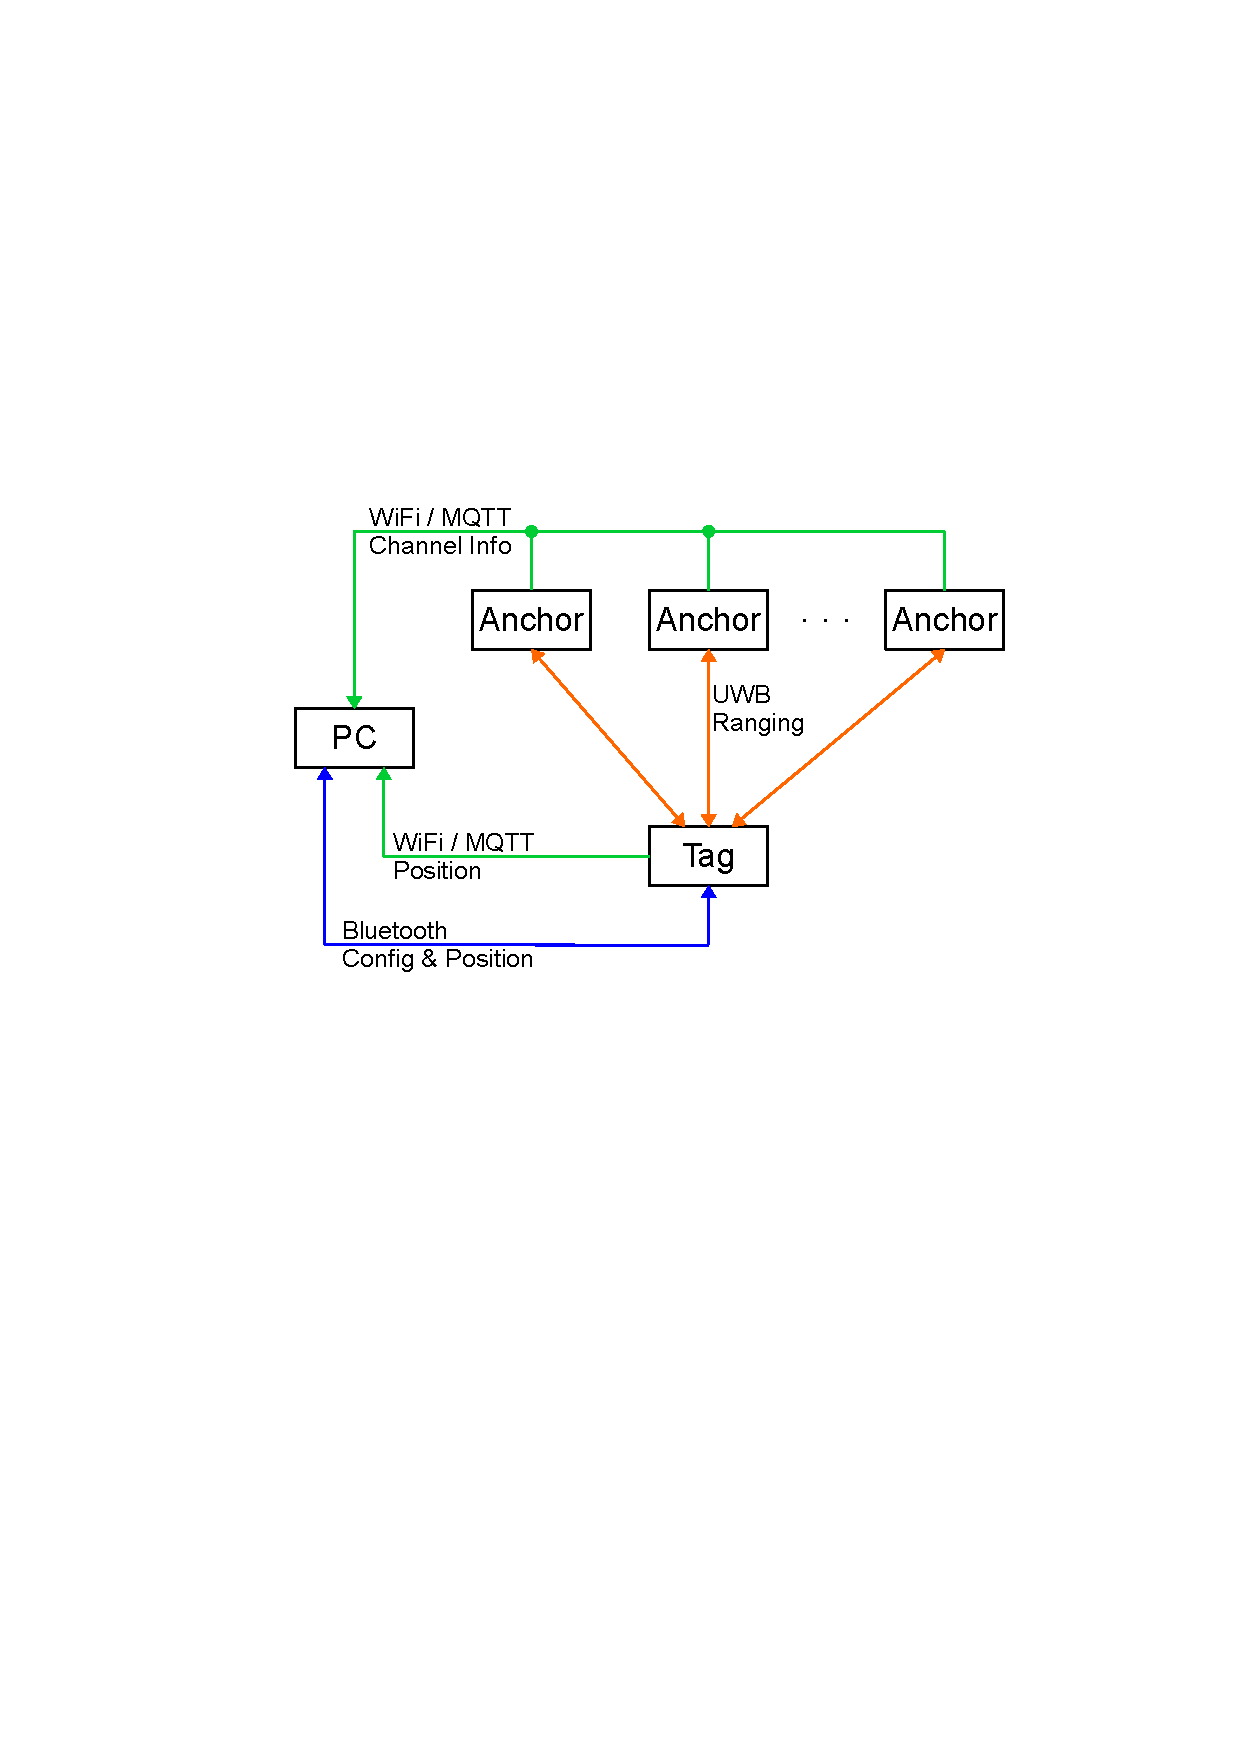
\includegraphics[width=0.6\textwidth]{pictures/information_flow.pdf}
	\caption{Sketch of the complete setup.}
	\label{fig:information_flow}
\end{figure}













\chapter{Main File Structure}
This chapter outlines the structure and organization of the main.cpp file of the UWB Project that runs on all of the UWB devices.

\section{Identification Parameters}
All UWB devices, irrespective of their function as anchors or tags, utilize the same codebase during the flashing process. 
The differentiation between these devices relies on two critical parameters configured during the initial flashing procedure. 
These parameters serve a dual purpose: defining the device's role as a tag or anchor and assigning a unique device identifier.
\vspace{4pt}
\newline
In essence, these parameters not only dictate whether a device acts as a tag or an anchor but also bestow each device with a distinctive identifier, enabling them to autonomously determine their respective addresses. 
This configuration approach ensures versatility and individuality among the UWB devices while maintaining a unified codebase.

\subsection{Set Identification Parameters}
The configuration of each device is primarily defined by two key parameters: the device ID and its designated role. 
To establish these parameters, a setup process is executed through the preproduction\_eeprom\_settings function, which is integrated into the setup section of the main.cpp file. 
This function accepts the current role and device ID as uint8\_t variables and records them in the EEPROM memory at an arbitrary position.
\vspace{4pt}
\newline
It is important to note that this setup process should only be performed once per device, typically during the initial configuration. 
Once the parameters are set and saved in the EEPROM, there is no need to invoke the preproduction\_eeprom\_settings function again during subsequent flashing processes unless a change in device configuration is desired. 
This approach streamlines the device setup procedure and ensures the persistence of the specified parameters across device power cycles.

\subsubsection{Role}
The role parameter is pivotal in determining whether a device functions as a tag or an anchor within the system. 
This parameter is stored in the EEPROM memory at address 0 and is represented by a binary value of 0 or 1. 
Throughout the codebase, this parameter is accessed and utilized through the IS\_INITIATOR constant.
\vspace{4pt}
\newline
If the value stored at EEPROM address 0 is 1, the device is configured to act as a tag. 
In this mode, it typically takes on the role of initiating UWB messages and serves specific functions accordingly. Conversely, if the value is 0, the device operates as an anchor. 
In this capacity, it primarily responds to incoming UWB messages, contributing to the overall UWB system by providing reference points and data to other devices.
\vspace{4pt}
\newline
This parameterization approach allows for dynamic role assignment and behavior based on a single value, making the system flexible and adaptive to the needs of each device.

\subsubsection{Device ID}
The device ID is also stored in the EEPROM, and it serves the crucial function of assigning a unique address to each device. 
This individualized addressing is essential for facilitating clear and unambiguous communication through UWB packages within the system. 
Each device must possess a distinct device ID to ensure that messages are accurately addressed to the intended recipient, and that devices can be uniquely identified in the network.
\vspace{4pt}
\newline
By storing the device ID in EEPROM, the ID can persist across power cycles and reboots, maintaining consistent identification for each device in the system. 
This approach is vital for seamless and reliable communication and data exchange between UWB devices, ensuring that messages reach their intended destinations without ambiguity.

\subsection{Address}
To ensure the secure and accurate encryption of UWB packages using the Advanced Encryption Standard (AES), each device requires a unique 32-bit address. 
This address is essential for enabling precise encryption and decryption processes. 
By encrypting a message with the destination address, the system guarantees that only the designated receiver can successfully decrypt the message. 
As a result, every device, both anchors and tags, must be aware of their own unique address.
\vspace{4pt}
\newline
For anchors, their individual addresses are directly determined by their respective device IDs. 
Each anchor selects its address from a predefined list based on its specific device ID. 
In contrast, the address for tags remains constant and is universally known across all devices as the global constant INITIATOR\_ADDR. 
This address assignment methodology ensures that each device can securely encrypt and decrypt messages using the appropriate addresses, contributing to the overall data security and integrity of the UWB communication system.

\section{User Input}
User input to change the current operating mode is facilitated through User Button 1. 
By associating an interrupt with this button, the ble\_kill\_flag is set, and the current\_mode variable is updated accordingly. 
For a comprehensive understanding of how these components are managed, please refer to section \ref{sec:Ble_Task}. 
This section will delve into the specifics of how the interrupt, ble\_kill\_flag, and current\_mode variable interact to facilitate seamless mode switching in the tag device's operation. 

\section{Main Variables}
\begin{itemize}
	\item \textbf{double distances[NUM\_LANDMARKS]}
	\newline
	This array stores the measured distances to landmarks, providing input for the Extended Kalman Filter (EKF) used for position estimation.
	It is constantly updated by an instance of the TofInitiator class. 
	
	\item \textbf{uint8\_t ble\_kill\_flag}
	\newline
	A flag used to control the operation of the BLE-Task, allowing for a smooth transition between operational and config mode.
	
	\item \textbf{coordinate own\_position}
	\newline
	A coordinate structure that holds the estimated 3D position of the UWB device, which is continuously updated by the EKF-Task. 
	
	\item \textbf{DynamicJsonDocument latest\_rx\_diagnostics}
	\newline
	This JSON document stores the most recent diagnostics information received from other UWB devices. It is utilized in UWB anchor mode to share information to an MQTT broker.
	
	\item \textbf{uint8\_t current\_mode}
	\newline
	Represents the operating mode of the UWB device, distinguishing between config and operational mode. It is toggled based on user input and controls the execution of relevant tasks.
	
	\item \textbf{uwb\_addr dest\_addr\_list[]}
	\newline
	An array containing UWB addresses of responder devices. 
	In UWB initiator mode, this list is used for initiating TOF measurements with multiple responder devices.
	
	\item \textbf{Task handles (ekf\_task\_handle, tdoa\_task\_handle, tof\_task\_handle, ble\_task\_handle, mqtt\_task\_handle)}
	\newline
	These handles are used to manage and control the execution of different FreeRTOS tasks responsible for specific functionalities in the UWB device.
\end{itemize}

\section{Main Functions}
\label{sec:Main_Functions}

\subsection{setup}
\label{subsec:setup}
The setup function in the UWB device code serves as the initialization routine that is run first when the ESP32 is powered on. 
It begins by configuring serial communication for debugging and EEPROM for persistent data storage. 
The pin where the user button 1 is connected to is set as an input and the user\_1\_button function is attached to it as an interrupt routine. 
Furthermore the three pins for the user LEDs are defined as output and all set to zero upon initialization. 
The current mode is set to "uwb\_mode" and the MQTT- as well as the TOF-Task are started. 
\vspace{4pt}
\newline
The function then checks if the device, it is running on, is defined as an initiator. 
If so the BLE- and EKF-Task are started as well. 
\vspace{4pt}
\newline
If the device is defined as a responder, it reads the JSON file named 
\newline
"uwb\_diacnostic\_type.json" from the SPIFFS on the ESP32.
It then creates a DynamicJsonDocument object (latest\_rx\_diagnostics) with three times the size of the JSON file, providing extra space for storing communication channel data.
The code proceeds to deserialize the contents of the JSON file into the latest\_rx\_diagnostics object. If there's an error during deserialization, it prints an error message to the serial monitor; otherwise, it indicates successful insertion of the JSON template. The file is then closed. Finally, the device ID is retrieved from EEPROM, and the "DeviceId" field in the latest\_rx\_diagnostics JSON document is set to this device ID so the MQTT broker can tell where from what responder the data originated. 

\subsection{void user\_1\_button}
\label{subsec:user_1_button}
The user\_1\_button function serves as an interrupt routine arrached to the user button 1. 
First the interrupt is detached. 
If the device is an initiator and in uwb\_mode it will toggle the ble\_kill\_flag and set to current mode to ble\_mode. 
If it is in ble\_mode it will toggle the ble\_kill\_flag and set to current mode to uwb\_mode. 
Lastly the interrupt gets attached back to the user button 1. 

\subsection{void animate\_leds}
\label{subsec:animate_leds}
This function sequentially illuminates and extinguishes LEDs in a predefined pattern, creating a visual animation. 
It provides a quick and noticeable indication of a specific mode. 
The LEDs involved in the animation are connected to GPIO pins on the ESP32. 

\subsection{void preproduction\_eeprom\_settings}
\label{subsec:preproduction_eeprom_settings}
This function takes two parameters - dev\_id representing the unique device identifier and is\_initiator indicating whether the device operates as an initiator or not. 
It writes these values into EEPROM, ensuring that the correct device ID and role information are stored persistently. This initialization process is crucial for the proper functioning of other tasks and functionalities in the UWB device, as they depend on the settings retrieved from EEPROM.

\subsection{Freertos Tasks}
\label{subsec:Freertos_Tasks}
The functions for the TOF-, MQTT-, BLE-, and EKF-Task are handeled by FreeRTOS to ensure concurrent and parallel execution of those functionalities within the device since they are the most critical to the operation. 
There functions are handled separately in the sections \ref{chap:tof_task} - \ref{sub:MQTT_Task}. 

\section{Scheduler}
\label{sec:Scheduler}
To efficiently measure distances to multiple anchors simultaneously, calculate their respective positions, and transmit the data to the software running on the devices, a scheduling system is implemented. 
This scheduling system is powered by the FreeRTOS library, an open-source real-time operating system, which leverages the dual-kernel capabilities of the ESP32 microcontroller.
\vspace{4pt}
\newline
The dual-kernel architecture ensures that critical tasks, like estimating distances, remain uninterrupted, reducing the risk of producing corrupted data. 
All tasks are initialized, started, and halted within the 'main.cpp' file, creating a well-structured and organized framework for managing these essential operations.

\subsection{TOF\_Task}
\label{chap:tof_task}

In the context of TOF-Task, it plays a pivotal role in the overall system, particularly in the domain of Time-of-Flight (TOF) distance measurement and positioning. This section outlines the primary functions of TOF-Task in a narrative form.
\vspace{4pt}
\newline
The initial task for TOF-Task is to identify the device's role within the system, specifically whether it should operate as a TofInitiator or a TofResponder. This role assignment is crucial as it dictates the device's behavior and responsibilities throughout the entire process.
\vspace{4pt}
\newline
Once the device's role is established, TOF-Task proceeds to create an instance of the appropriate object, either TofInitiator or TofResponder, and initializes it. This instantiated object assumes the critical responsibility of managing the distance measurement process.
\vspace{4pt}
\newline
At the core of TOF-Task's operation lies the facilitation of distance measurements. If the device takes on the role of a responder, it remains in a passive stance during the measurement process, awaiting initiation from another device. Conversely, when the device serves as an initiator, it leads the way in conducting distance measurements.
\vspace{4pt}
\newline
In scenarios where the device functions as the initiator, a crucial user feedback mechanism comes into play. User LED 1 is activated to provide visual feedback, signaling that this particular device is taking the initiative in distance measurement and position estimation. Such feedback proves invaluable, especially in systems involving multiple devices, ensuring users are aware of which device is actively involved in determining the position.
\vspace{4pt}
\newline
For the initiator role, TOF-Task manages the storage of calculated distances. These distances, representing measurements to each anchor, are stored within the "double distances[]" array. This array serves as a vital source of information for the subsequent stages of the positioning algorithm.
\vspace{4pt}
\newline
In summary, TOF-Task serves as the central orchestrator, dynamically allocating roles to devices as initiators or responders and configuring the corresponding objects to execute distance measurements. This dynamic allocation of tasks ensures the effective functioning of the system, and when necessary, it offers user feedback to enhance the transparency of the positioning process.

\subsection{EKF-Task}
The EKF task is a critical component of the system, running exclusively on the tag device. 
Its primary purpose is to leverage the information provided by the "double distances[]" array, which contains the distances to all available anchors. 
With this data, the EKF task performs calculations to estimate the tag's position. 
This estimation process is triggered every time when all landmark distances are covered, ensuring that the system continually updates its understanding of the tag's location.
\vspace{4pt}
\newline
The EKF algorithm, a cornerstone of this task, incorporates statistical techniques and dynamic models to refine the accuracy of the position estimate. 
By doing so, it can effectively handle factors like noise and uncertainties, making it a robust solution for real-time positioning.
\vspace{4pt}
\newline
Once the EKF-task completes its calculations, the resulting X and Y coordinate values are transmitted through the UART interface and via MQTT.  
\vspace{4pt}
\newline
For a comprehensive understanding of the theory and principles that underpin the Extended Kalman Filter and its role in this system, you'll find in-depth coverage in Chapter \ref{chap:EKF_Handling}. 
This chapter will delve into the mathematical and conceptual foundations of the EKF, ensuring that readers gain a clear grasp of how it operates and contributes to the overall functionality of the system.

\subsection{BLE\_Task}
\label{sec:Ble_Task}
Similar to the EKF-Task, the BLE-Task is designed to run exclusively on the tag device, and it serves two primary objectives.
\vspace{4pt}
\newline
The first objective is to facilitate device configuration, a process carried out through Bluetooth connectivity with the dedicated ``UWB Configuration`` desktop software. This configuration process entails defining the coordinates of each anchor device and saving these values in the device's EEPROM. A comprehensive guide on how to connect the tag device with the desktop software can be found in the UWB User Guide.
\vspace{4pt}
\newline
The second objective of the BLE-Task is to relay the current position of the tag device via Bluetooth to the corresponding desktop software. The software then plots these positions in an X-Y coordinate system, providing a real-time visual representation of the tag's movements.
\vspace{4pt}
\newline
When the BLE-Task is first initialized, it instantiates the BleConfigLoader class. The workings of this class, along with the broader Bluetooth management process, will be expounded upon in the forthcoming chapter, referenced as \ref{chap:Bluetooth_Handling}.
\vspace{4pt}
\newline
The tag device operates in two distinct modes saved in the current\_mode variable. The first is the uwb\_mode, which serves as its standard operating mode. In this mode, the device performs distance measurements, calculates its own position, and transmits this information via UART, as previously described in \ref{chap:tof_task}.
\vspace{4pt}
\newline
The other operational mode is the ble\_mode, which is exclusively focused on maintaining a connection with the desktop software. 
In this mode the device waits for the trigger from the UWB Configuration software to take in the newly inputted anchor positions and save them into the EEPROM. 
It also outputs the currently saved anchor positions so that they can be displayed and changed in the UWB Configuration desktop software. 

\subsubsection{Output current position}
In the default startup scenario, where the uwb\_mode is automatically selected without any additional user input, the BLE-Task is responsible for taking the currently estimated position from the global own\_position variable and transmitting it via Bluetooth. 
This transmission is achieved using the send\_position method of the BleConfigLoader class. Detailed insight into the functionality of this process will be provided in the forthcoming chapter, referenced as \ref{chap:Bluetooth_Handling}.
\vspace{4pt}
\newline
This continuous updating procedure persists indefinitely, with the current position being sent repeatedly, unless the ble\_kill\_flag is triggered. 
The flag is set when a user initiates a mode change to ble\_mode by pressing user button 1.
\vspace{4pt}
\newline
This mode-switching functionality ensures that the device can seamlessly transition between its primary operating modes based on user input. 

\subsection{MQTT\_Task}
\label{sub:MQTT_Task}
The MQTT\_Task function handles all the MQTT communication. 
It first determines if it is run by the tag or any responder and figuring out its device ID by reading the EEPROM. 
Then it creates a string identifier (String clientId) containing its device ID so the MQTT messages can be told apart from where they originated from. 
\vspace{4pt}
\newline
Subsequently, the function creates an instance of the MqttClient class, encapsulating the essential functionality for MQTT communication. 
This includes setting up the MQTT topic ("uwb\_devices"), specifying the MQTT server details, providing WiFi credentials, and configuring a buffer size for efficient data handling.
\vspace{4pt}
\newline
Within the core of the function lies an infinite loop that serves as the heartbeat of the MQTT communication task. 
The primary objective of this loop is to ensure the persistent operation of the MQTT client. 
Consequently, the mqttClient.update() method is called at every iteration, allowing the client to handle incoming messages and maintain the MQTT connection.
\vspace{4pt}
\newline
As part of the communication strategy, the MQTT\_Task function publishes messages to specific MQTT topics based on the device's role. 
In cases where the device is an initiator (is\_initiator = 1), it publishes position information, formatted as a JSON string, to the "tag/{dev\_id}/position" topic. 
Conversely, if the device is not an initiator (is\_initiator = 0), it publishes UWB diagnostics information, serialized into JSON, to the "anchor/{dev\_id}/uwb\_info" topic.
\vspace{4pt}
\newline
This task structure enables the integration of the device into a larger Ultra-Wideband (UWB) communication system. 
It showcases the capability to disseminate critical information, such as device positions or UWB diagnostics, via the MQTT protocol. 
The inclusion of delays between message publications controls the communication frequency, aligning with the specific requirements of the UWB communication system. 

\subsubsection{Configuration}
When the user triggers a mode change to ble\_mode by pressing button 1, the ble\_kill\_flag is activated, which effectively terminates the loop responsible for continuously transmitting the current position.
\vspace{4pt}
\newline
In the ble\_mode, the device first retrieves its current configuration, encompassing all previously saved anchor positions, from the EEPROM. This retrieval process is achieved through the load\_config\_from\_eeprom method of the BleConfigLoader class. 
Subsequently, the device compiles this configuration data into a string formatted as a JSON object and transmits it via Bluetooth, using the save\_config\_to\_ble method. 
This JSON-formatted data includes the anchor positions.
\vspace{4pt}
\newline
Following this configuration update transmission, a new loop commences. In this loop, the device continually receives the most up-to-date anchor positions sent from the configurator device via Bluetooth. 
These positions are then saved locally on the tag device, and the new anchor configuration is conveyed back to the configurator device, ensuring that the positions are received and updated accurately.
\vspace{4pt}
\newline
In addition to this configuration exchange, the animate\_leds function is invoked, causing the user LEDs to flash in a distinct pattern. 
This visual feedback serves as an indicator to the user that the device is in Bluetooth configuration mode.
\vspace{4pt}
\newline
The configuration loop persists until the "Save Config" button is pressed within the UWB Configuration desktop GUI. 
This action initiates the sending of a character to the tag device, triggering the save\_config\_to\_eeprom method. 
This method is responsible for writing the updated anchor coordinates into the EEPROM of the device and subsequently restarting the device with the new configuration in place. 
This completes the process of updating and saving anchor positions for the tag device during its operation in ble\_mode.




\chapter{UWB Handling}

\section{Distance Measurement}
The distance measurements in this system are conducted using a Time-of-Flight (ToF) methodology. This means that the time taken for an Ultra-Wideband (UWB) message to be transmitted from one device and received by another is a crucial factor. By subtracting the time when the UWB message is transmitted from the time it is received, we obtain the flight time. This represents the duration it took for the electromagnetic field to propagate from the sender to the receiver. This time is typically measured in seconds.
\vspace{4pt}
\newline
To derive the distance between the two UWB devices, this time is multiplied by the approximate velocity at which these electromagnetic fields expand. In a perfect vacuum, this velocity would equal the speed of light, which is 299,792,458 meters per second, often denoted as 'c'. However, under atmospheric conditions where this setup operates, the speed of light is slightly slower. Therefore, in this setup, an approximated speed of 299,702,547 meters per second is used. 
\vspace{4pt}
\newline
It's worth noting that the accuracy of the time measurement is crucial since even a small error in this time measurement can result in a relatively significant error in distance estimation. To ensure precise time measurements, the DW3000 IC requires a highly accurate clock signal with minimal drift. The DWM3000 module offers an advantage in this regard, as it already integrates the DW3000 chip with an on-module oscillator suitable for UWB operations.
A visual representation of the ToF distance calculation process is depicted in Figure \ref{fig:tof_sketch}.

\begin{center}
	\begin{figure}[!hbt]
		\centering
		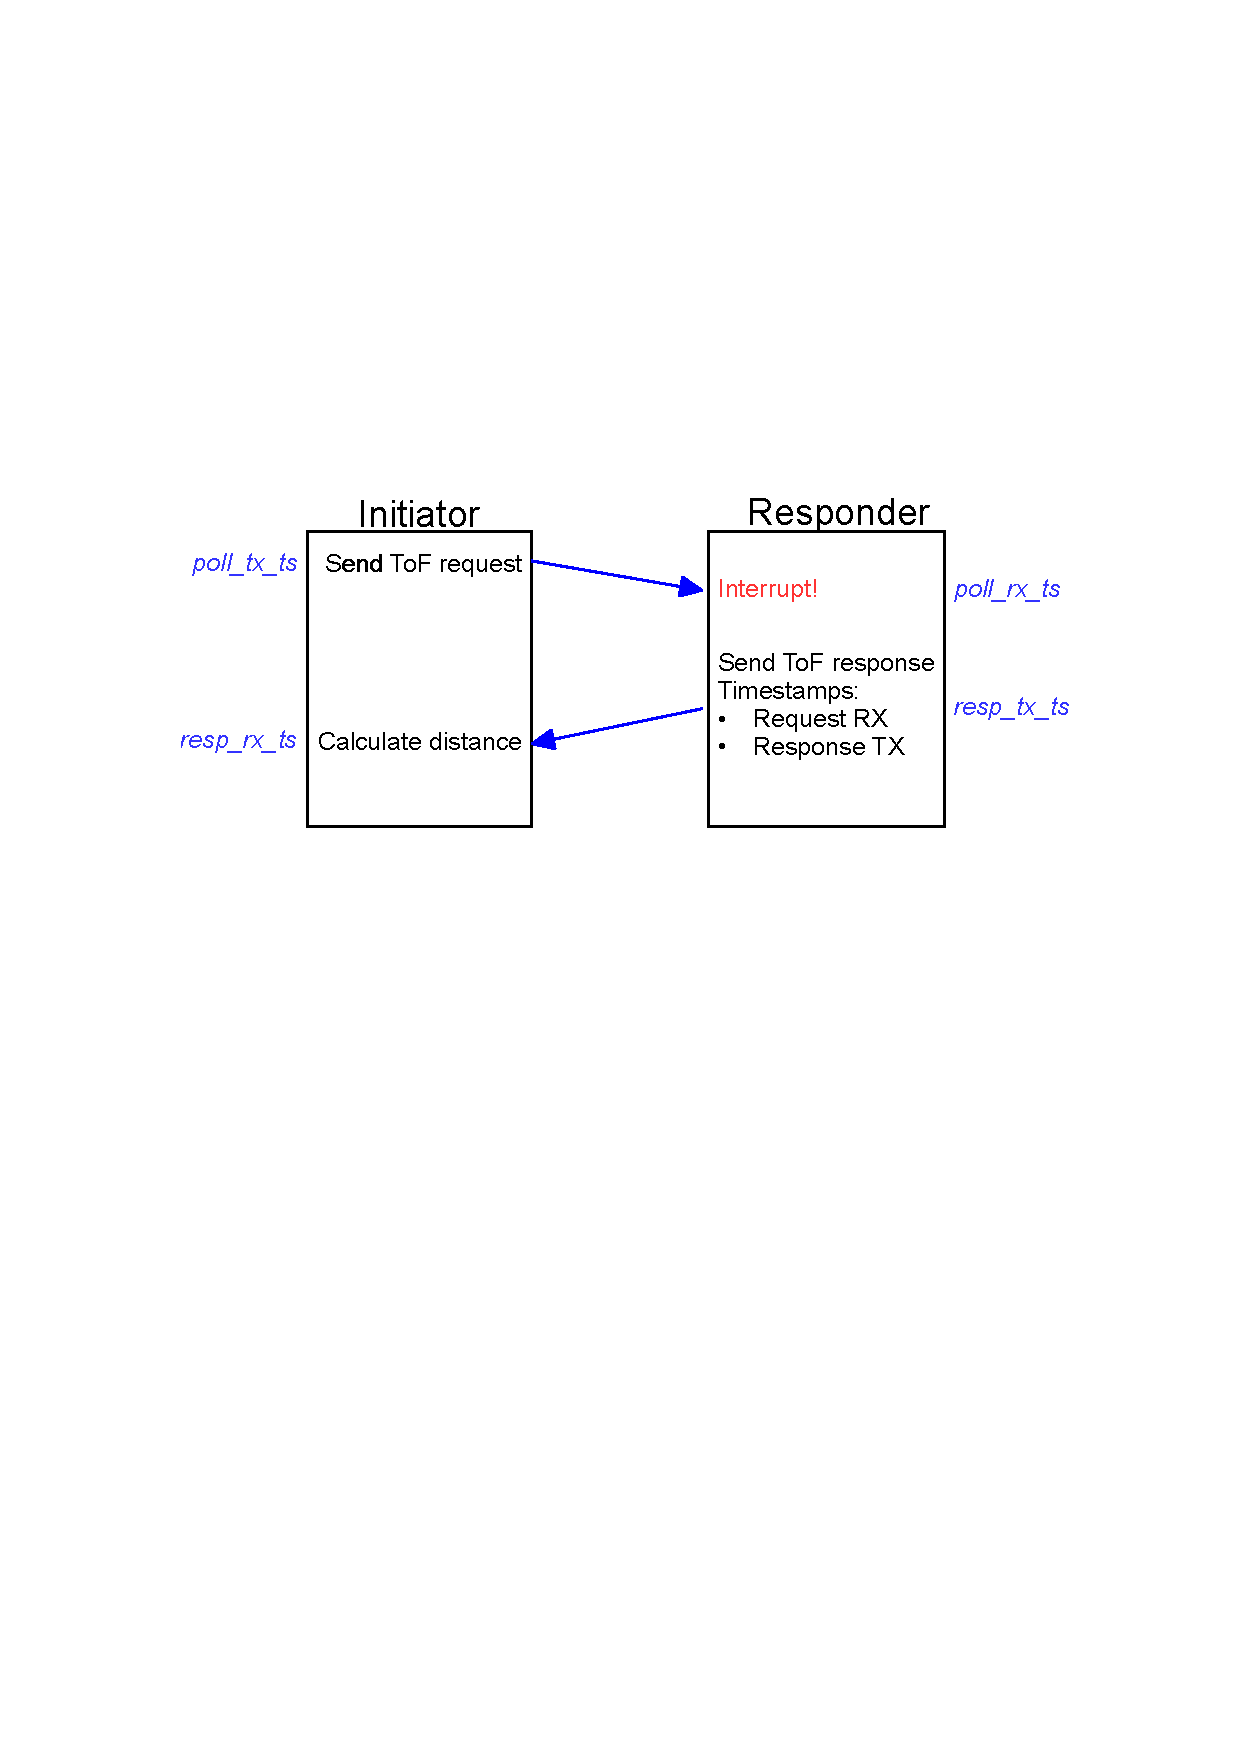
\includegraphics[width=0.8\textwidth]{pictures/ToF_scheme.pdf}
		\caption{Sketch of the complete setup.}
		\label{fig:tof_sketch}
	\end{figure}
\end{center}


To estimate the distance, four timestamps, marked in blue in Figure \ref{fig:tof_sketch}, are used. These timestamps are expressed in ticks and are stored in a 32-bit variable. The timestamps are as follows:

\begin{center}
	\begin{table}[!hbt]
		\begin{tabular}{ | m{5em} | m{10cm} |} 
			\hline
			poll\_tx\_ts & Time of request being sent by Initiator \\ 
			\hline
			poll\_rx\_ts & Time of request being received by Responder \\ 
			\hline
			resp\_tx\_ts & Time of response being sent by Responder \\ 
			\hline
			resp\_rx\_ts & Time of response being received by Initiator \\ 
			\hline
		\end{tabular}
		\caption{Timestamp variables.}
		\label{tab:timestamps}
	\end{table}
\end{center}

To calculate the time it took for the poll message to travel from the initiator to the responder, the \blueconsolas{poll\_tx\_ts} timestamp is subtracted from the \blueconsolas{poll\_rx\_ts} timestamp, yielding the \blueconsolas{rtd\_init} value. Similarly, for the time the response message took to travel in the opposite direction, \blueconsolas{resp\_tx\_ts} is subtracted from \blueconsolas{resp\_rx\_ts}, resulting in the \blueconsolas{rtd\_resp} variable.
\vspace{4pt}
\newline
To determine the distance between the initiator and the responder, the two times (\blueconsolas{rtd\_init} and \blueconsolas{rtd\_resp}) are averaged. Before averaging, the response time (\blueconsolas{rtd\_resp}) is adjusted by applying an offset factor (1 - clockOffsetRatio). This compensates for potential variations that may arise if the clock of the initiator runs slightly faster or slower than the responder due to factors such as aging effects, temperature, voltage, or manufacturing discrepancies.
\vspace{4pt}
\newline
Finally, to compute the distance between the two devices, the average time is converted to seconds and then multiplied by the predefined speed of light, representing the speed of electromagnetic field expansion.
\vspace{4pt}
\newline
This process is subsequently repeated for all of the saved anchors to get the distance to every single one. 
The calculated distances are saved in the distances array. 



\section{TofDevice}
\label{sec:TofDevice}
The TofDevice class is a base class for Tof devices, serving as a superclass for both TOF initiators and responders. 
It encapsulates common functionality and configurations required for TOF devices using the DW3000 chip.
The class provides methods for initializing and configuring the TOF device, starting a watchdog timer for handling failure events, enabling LEDs for debugging, and implementing the main loop for the TOF device.
Additionally, it includes parameters and configurations specific to the DW3000 chip, such as communication settings, encryption keys, and antenna delay values.

\subsection{TofDevice Variables}
\label{subsec:TofDevice_Variables}

\subsubsection{Constants}
\begin{itemize}
	\item \textbf{DEST\_PAN\_ID}
	\newline
	desc
	\item \textbf{START\_RECEIVE\_DATA\_LOCATION}
	\newline
	desc
	\item \textbf{ALL\_MSG\_SN\_IDX}
	\newline
	desc
	\item \textbf{RESP\_MSG\_POLL\_RX\_TS\_IDX}
	\newline
	desc
	\item \textbf{RESP\_MSG\_RESP\_TX\_TS\_IDX}
	\newline
	desc
	\item \textbf{RESP\_MSG\_TS\_LEN}
	\newline
	desc
	\item \textbf{INITIATOR\_KEY\_INDEX}
	\newline
	desc
	\item \textbf{RESPONDER\_KEY\_INDEX}
	\newline
	desc
	\item \textbf{RX\_BUF\_LEN}
	\newline
	desc
	\item \textbf{TX\_ANT\_DLY}
	\newline
	desc
	\item \textbf{RX\_ANT\_DLY}
	\newline
	desc
\end{itemize}

\subsubsection{Private Variables}
\begin{itemize}
	\item \textbf{Watchdog my\_watchdog}
	\newline
	The my\_watchdog variable is an instance of the Watchdog class, representing a software watchdog timer used to monitor the proper execution of the TOF device's main loop. It is initialized with a timeout value, and its purpose is to reset the device if the timer is not reset within the specified duration, enhancing the device's reliability and fault tolerance. The section\ref{sec:Watchdog_Handling} delves into the watchdog class.
	
	\item \textbf{uwb\_addr src\_address}
	\newline
	The src\_address of type long long holds a 32-Bit UWB address. 
	
	\item \textbf{String type}
	\newline
	The type variable of type String holds the information whether the device is identified as tag or responder. 
	
	\item \textbf{mac\_frame\_802\_15\_4\_format\_t mac\_frame}
	\newline
	The mac\_frame variable is of the type mac\_frame\_802\_15\_4\_format\_t and used to construct and alter the UWB message corresponding to the IEEE 802.15.4 communication standard. 
	
	\item \textbf{uint8\_t poll\_msg[4]}
	\newline
	poll\_msg is a four byte array representing the specific poll message payload. 
	In this case it is labeled {'P', 'o', 'l', 'l'} and is used by the tag ot initiate a UWB cycle. 
	
	\item \textbf{uint8\_t resp\_msg[16]}
	\newline
	The resp\_msg is similar to the poll\_msg used to construct MAC frames. 
	In this case the message is 16 bytes ling with the first 8 bytes reserved for the timestamps of the responder. The last 8 bytes carry the characters 'R', 'e', 's', 'p', 'o', 'n', 's', 'e' indicating the nature of the message. 
	
	\item \textbf{uint8\_t rx\_buffer[RX\_BUF\_LEN]}
	\newline
	The rx\_buffer array allocates memory to store a incoming UWB message of the maximum size. 
	
	\item \textbf{uint32\_t status\_reg}
	\newline
	The status\_reg holds information about the process of a message being sent. 
	It masks errors and timeouts that may occur when a UWB message is transmitted or received. 
	
	\item \textbf{dwt\_aes\_job\_t aes\_job\_tx, aes\_job\_rx}
	\newline
	Both aes\_job\_tx and aes\_job\_rx are of the struct type dwt\_aes\_job\_t and contain information needed for the AES encryption/decryption of each MAC frame being send or received. 
	
	\item \textbf{int8\_t status}
	\newline
	The status variable is used to save and evaluate the status of a AES encryption. It masks different AES errors to its bits. 
	
	\item \textbf{dwt\_aes\_config\_t aes\_config}
	\newline
	The aes\_config variable represents an instance of the dwt\_aes\_config\_t type. 
	It is used to configure and specify parameters for the AES operations within the TOF device. 
	The dwt\_aes\_config\_t type includes fields for selecting the AES core type, setting the key source, and defining other encryption-related configurations. 
	
	\item \textbf{dwt\_config\_t config}
	\newline
	The config variable is an instance of the dwt\_config\_t type, and it is used to store configuration parameters related to the DW3000 chip, which is used for TOF communication. 
	The dwt\_config\_t type includes fields such as channel number, preamble length, data rate, and other settings that determine the behavior of the DW3000 chip during communication. 
	This variable is utilized in the setup process to initialize and configure the TOF device for proper operation.
	
	\item \textbf{dwt\_aes\_key\_t keys\_options[NUM\_OF\_KEY\_OPTIONS]}
	\newline
	The keys\_options variable in the TofDevice class is an array of dwt\_aes\_key\_t elements. 
	It is used to store different encryption keys for AES operations within the TOF device. 
	Each element in the array (dwt\_aes\_key\_t) represents a set of encryption keys, allowing for multiple key options. 
	These keys are used to secure communication between TOF devices, providing a level of cryptographic protection for the transmitted data.
\end{itemize}

\subsection{TofDevice Constructor}
\label{subsec:TofDevice_Constructor}
The TofDevice constructor initializes a new instance of the TofDevice class within the Device namespace. It takes two parameters: uwb\_addr src for the source address of the TOF device and unsigned long wdt\_timeout for the watchdog timer's timeout duration. 
It begins by initializing SPI comminication to the DWM3000 chip and ensuring that it is in a stable state after startup through a soft reset and a brief delay. 
Subsequently, it checks the device's idleness in the Idle RC state before proceeding. 
The method then initializes the DW3000 chip using the dwt\_initialise function. 
If any of these steps fail, it prints error messages and enter a loop indicating failure. 
Lastly the config data for the operation of the DWM and the AES encryption as well as are the keys\_options set in the corresponding variables config, aes\_config and keys\_options are set

\subsection{virtual void setup}
\label{subsec:TofDevice_setup}
The setup method in the TofDevice class serves as the initialization routine for the TOF device. 
It uses the dwt\_configure function to configure the DWM3000 with the config options set in the constructor describes in \ref{subsec:TofDevice_Constructor}. 
If this fails it will print an error message and go in a loop. 
The configuration of the transmission spectrum parameters is handled by dwt\_configuretxrf, and default antenna delay values are applied through dwt\_setrxantennadelay and dwt\_settxantennadelay. 

\subsection{void start\_wdt}
\label{subsec:TofDevice_start_wdt}
The start\_wdt method in the TofDevice class initiates the watchdog timer associated with the TOF device using the begin method of the Watchdog class targeted in \ref{subsec:Watchdog_begin}. This method is responsible for commencing the timer, which monitors the execution of the device's main loop. 

\subsection{void enable\_leds}
\label{subsec:TofDevice_enable_leds}
The enable\_leds method activates the RX and TX LEDs for debugging purposes. 
By enabling the LEDs, each transmission triggers a visual indication of sent and received messages, aiding in the debugging process. Note that in practical low-power applications, LEDs might be disabled to conserve power, but in a debug scenario or when the device is hooked up to a stable supply like the main grid. 

\subsection{virtual void loop}
\label{subsec:TofDevice_loop}
The loop method represents the main operational loop for the TOF device. 
Within this loop, the device continually resets the watchdog timer using the resetTimer method, ensuring that the device remains within its expected operational timeframe. 

\subsection{char* get\_type}
\label{subsec:TofDevice_get_type}
The private get\_type method returns a pointer to the type variable of the TOF device seen in \ref{subsec:TofDevice_Variables}, offering a descriptive label for the TOF device's classification.

\section{TofInitiator}
\label{sec:TofInitiator}
The TofInitiator class is a subclass of TofDevice and represents a TOF initiator device. 
It extends the base class functionality to handle TOF request transmissions, response processing, and secure communication with responder devices. 
The class encapsulates frame construction, nonce generation, and specific logic for managing communication with multiple responders.

\subsection{TofInitiator Variables}
\label{subsec:TofInitiator_Variables}

\subsubsection{Extern Variables}
\begin{itemize}
	\item \textbf{extern double distances[NUM\_LANDMARKS]}
	\newline
	The distances variable is an external array declared as extern double 
	\newline
	distances[NUM\_LANDMARKS] in the tof-initiator.h file. 
	This array is initialized in ther main.cpp file and is intended to store distance measurements calculated by the TOF initiator for each responder in the system. 
	The size of the array, NUM\_LANDMARKS, is determined by the number of responders in the system, and each element in the array holds the calculated distance for a specific responder. 
	The actual values are be updated during the processing of TOF responses in the process\_tof\_response method as described in \ref{subsec:TofInitiator_process_tof_response}.
\end{itemize}

\subsubsection{Private Variables}
\begin{itemize}
	\item \textbf{uint32\_t frame\_cnt}
	\newline
	The frame\_cnt variable represents the frame count, tracking the number of frames transmitted by the TOF initiator. 
	It is incremented after each transmission and is used to manage frame sequencing within the communication protocol. 
	This count helps maintain synchronization and order in the communication between the initiator and responder devices.
	
	\item \textbf{seq\_cnt}
	\newline
	The seq\_cnt variable represents the frame sequence number, and it is used to keep track of the sequence of frames transmitted by the TOF initiator. 
	It is incremented after each transmission to ensure that each frame has a unique identifier within the communication protocol. 
	The seq\_cnt value is part of the frame's metadata and aids in maintaining order and synchronization between the initiator and responder devices in the TOF communication system.
	
	\item \textbf{uint8\_t nonce[13]}
	\newline
	The nonce variable is a 13-byte array used as a nonce (Number used Once) in the context of secure communication. 
	It serves as a unique value for each frame transmission and is utilized in the encryption and decryption processes to enhance security by preventing replay attacks. 
	The nonce is generated and updated for each TOF frame transmission, contributing to the integrity of the communication between the TOF initiator and responder devices.
	
	\item \textbf{dst\_address}
	\newline
	The dst\_address variable is a pointer to an array of destination addresses for the responders. 
	It represents the target addresses to which the TOF initiator sends its requests. 
	The array holds the addresses of all individual responder devices, and the TofInitiator class uses this information to selectively communicate with each responder one after another during the TOF communication process.
	
	\item \textbf{uint8\_t total\_responders}
	\newline
	The total\_responders variable represents the total number of responder devices that the TOF initiator communicates with. 
	It indicates the size of the array of destination addresses (dst\_address) and helps manage the looping through responder devices during the TOF communication process. 
	The TOF initiator iterates through the responders, sending TOF requests and processing responses, and total\_responders determines the number of devices in this communication setup.
	
	\item \textbf{uint8\_t current\_responder}
	\newline
	The current\_responder variable is an index used to keep track of the current responder being communicated with during the TOF communication process. 
	It is incremented and looped to iterate through the array of destination addresses (dst\_address), allowing the TOF initiator to selectively send TOF requests and process responses from different responder devices. 
	This index management facilitates sequential communication with multiple responders within the specified array.
	
	\item \textbf{double tof}
	\newline
	The tof variable represents the calculated Time-of-Flight for a particular communication instance. 
	It is used to store the calculated time it takes for a signal to travel from the TOF initiator to the responder and back. 
	The tof value is derived during the processing of TOF responses and is an essential parameter for determining the distance between devices using the speed of light.
	
	\item \textbf{double temp\_distance}
	\newline
	The temp\_distance variable is used to buffer the calculated distance based on the Time-of-Flight measurement during the processing of TOF responses. 
	It represents a temporary variable for storing the distance information before it may be further utilized in the application. 
\end{itemize}

\subsection{TofInitiator Constructor/Dectructor}
\label{subsec:TofInitiator_Constructor}
The TofInitiator constructor takes parameters representing the source address for the TOF initiator (src), an array of destination addresses for the responders (dst), the watchdog timer timeout value (wdt\_timeout), and the number of responder devices (num\_of\_responders). 
It sets the type String variable to "Initiator" indicating its role, initializes tof, temp\_distance and frame\_cnt with 0 and seq\_cnt to 10 (0x0A). 
Latly the MAC-Frame is assembled. 

\subsection{virtual void setup}
\label{subsec:TofInitiator_setup}
The setup method initializes the TOF initiator by calling the base class's setup method to configure basic parameters descibed in \ref{subsec:TofDevice_setup}. 
It then sets the expected response delay and timeout using the dwt\_setrxaftertxdelay and dwt\_setrxtimeout functions. 
After that the parameters for the AES are set for rx encryption and tx decryption. 

\subsection{virtual void loop}
\label{subsec:TofInitiator_loop}
The loop method serves as the central processing hub, orchestrating the continuous operation of the TOF initiator device. 
It begins by invoking the base class loop method, decribed in \ref{subsec:TofDevice_loop}, which includes resetting the watchdog timer to prevent system resets due to potential failures. 
\vspace{4pt}
\newline
Within the loop, the current\_responder index is iteratively updated, allowing the TOF initiator to cycle through the array of destination addresses. 
For each iteration, a TOF request is sent to the selected responder using the send\_tof\_request function. 
After sending the method checks certain bits in the status\_reg variable to ensure the message was being sent correctly and if so, updates the seq\_cnt and frame\_cnt counters. 
\vspace{4pt}
\newline
The method then enters a loop until it detects a response message being received by checking the SYS\_STATUS\_RXFCG\_BIT\_MASK masked in the status\_reg variable. 
Then the method processes the response by calling the process\_tof\_response described in \ref{subsec:TofInitiator_process_tof_response} and puts it in the distances array. 

\subsection{void send\_tof\_request TBE}
\label{subsec:TofInitiator_send_tof_request}
The send\_tof\_request method in the TofInitiator class is responsible for initiating and sending a Time-of-Flight (TOF) request to a specific destination address (responder). Here's a description without bullet points:

The send\_tof\_request method configures the necessary parameters, such as encryption keys and nonce, in preparation for the TOF request. It encrypts the TOF request payload using AES encryption, sets up the frame control, and triggers the transmission. The method ensures that the TOF initiator communicates securely with the designated responder, facilitating the exchange of information essential for subsequent TOF calculations.

\subsection{void process\_tof\_response TBE}
\label{subsec:TofInitiator_process_tof_response}
The process\_tof\_response method in the TofInitiator class is responsible for handling and extracting relevant information from a Time-of-Flight (TOF) response received from a responder device. Here's a description without bullet points:

The process\_tof\_response method begins by clearing the indication of a good received frame in the status register. It then reads the length of the received frame and proceeds to decrypt the payload of the response using AES decryption. The method validates and checks for potential errors in the decryption process.

Upon successful decryption, the method verifies that the received frame matches the expected response from the TOF responder. It extracts the relevant timestamps from the response payload, computes the Time-of-Flight (TOF) and distance based on these timestamps, and updates the tof and temp\_distance variables.

The process\_tof\_response method plays a crucial role in interpreting the TOF response, ensuring data integrity, and facilitating the accurate calculation of distances for localization or positioning purposes within the Time-of-Flight communication system.


\section{TofResponder}
\label{sec:TofResponder}

\subsection{TofResponder Variables}
\label{subsec:TofResponder_Variables}

\subsection{TofResponder Constructor/Dectructor}
\label{subsec:TofResponder_Constructor}

\subsection{virtual void setup}
\label{subsec:TofResponder_setup}

\subsection{virtual void loop}
\label{subsec:TofResponder_loop}

\subsection{void update\_rx\_diagnostics}
\label{subsec:TofResponder_update_rx_diagnostics}

\subsection{static void rx\_ok\_cb}
\label{subsec:TofResponder_rx_ok_cb}


\section{Watchdog Handling}
\label{sec:Watchdog_Handling}
To ensure that the UWB task on all devices keeps being up and running to deliver data for continuing to estimate the tag's position and is not interrupted or halted in an infinite loop a watchdog logic is implied in the TofDevice class. 
The watchdog is implemented in the "watchdog.h" and "watchdog.cpp" files. 
The timer used is given by FreeRTOS xTimer functionality. 

\subsection{Watchdog Variables}
\label{subsec:Watchdog_Variables}

\subsubsection{private Variables}
\begin{itemize}
	\item \textbf{unsigned long timeoutMillis}
	\newline
	Holds the duration in milliseconds after the watchdog will fire. 
	\item \textbf{TimerHandle\_t timer}
	\newline
	Holds FreeRTOS timer handle of type TimerHandle\_t. 
\end{itemize}

\subsection{Watchdog Constructor}
\label{subsec:Watchdog_Constructor}
When constructing a Watchdog object the constructor takes in the timeoutMillis variable of type unsigned long and assigns it. 

\subsection{void resetTimer}
\label{subsec:Watchdog_resetTimer}
The resetTimer Method takes in no parameters and resets the timer object of type TimerHandle\_t to 0 using the FreeRTOS xTimerReset function. 

\subsection{void begin}
\label{subsec:Watchdog_begin}
The begin Method creates the timer of type TimerHandle\_t using the FreeRTOS xTimerCreate fuction. 
It assigns the name "WatchdogTimer", the timeout period and the timerCallback method as a callback dunction that is fired once the designated time is elapsed. 
Then it is checked if the timer creation was successful and the timer is started using FreeRTOS function xTimerStart. 
If the timer creation as unsuccessful an error message will be outputted via UART. 

\subsection{void stop}
\label{subsec:Watchdog_stop}
The stop method checks if a timer object is present. 
If so it is stopped and deleted by the FreeRTOS functions xTimerStop and xTimerDelete. 

\subsection{unsigned long get\_timeout}
\label{subsec:Watchdog_get_timeout}
The get\_timeout method, when called, acts as a getter function and returns the current timeout period saved in the timeoutMillis variable of type unsigned long. 

\subsection{static void timerCallback}
\label{subsec:Watchdog_timerCallback}
The timerCallback function is called every time duration in timeoutMillis is elapsed. 
When called the function prints a serial message that the watchdog timer has elapsed and then restarts the esp device using the esp\_restart function. 

\chapter{MQTT Handling}
\label{chap:MQTT_Handling}

The MqttClient class is designed for managing MQTT communication in an ESP32-based Arduino environment. 
It encapsulates the functionality for establishing and maintaining a connection to an MQTT broker, handling incoming messages through a callback function, and publishing messages to specified MQTT topics. 
The class includes methods for checking the connection status, obtaining the MAC address of the associated WiFi client, and ensuring periodic updates to handle MQTT events.
The necessary information to establish the connection are set in the main file. 

\section{MqttClient Class}
\label{sec:MqttClient_Class}

%\vspace{4pt}
%\newline

\subsection{mqtt Variables}
\label{sub:mqtt_Variables}

\subsubsection{Private Variables}

\begin{itemize}
	\item \textbf{WiFiClient espClient}
	\newline
	The espClient is an instance of the WiFiClient class, which is part of the ESP32 Arduino core libraries. 
	This object is used to manage the WiFi connection on the ESP32 device. 
	The WiFiClient class provides methods for establishing, maintaining, and handling communication over a WiFi network.
	\vspace{4pt}
	\newline
	In the context of the MqttClient class, espClient serves as the WiFi client for the ESP32, allowing the device to connect to a WiFi network. 
	It is then utilized by the PubSubClient (MQTT client) to establish and maintain the MQTT connection over the WiFi network. 
	
	\item \textbf{PubSubClient client}
	\newline
	The client is an instance of the PubSubClient class, which is used to handle MQTT communication on the ESP32. 
	The PubSubClient library provides functionalities for interacting with MQTT brokers, allowing the ESP32 to both publish messages to specific topics and subscribe to topics to receive messages.
	\vspace{4pt}
	\newline
	In the context of the MqttClient class, the client object represents the MQTT client used for communication with an MQTT broker. 
	It is associated with the WiFiClient instance (espClient), which manages the underlying WiFi connection. 
	The client object is responsible for connecting to the MQTT broker, handling incoming messages, and publishing messages to specified topics.
	
	\item \textbf{String dev\_id}
	\newline
	dev\_id is a variable of type String, representing the device ID associated with the MQTT client instance. 
	It is passed as a parameter to the constructor and can be utilized for identification or customization purposes within the MQTT communication. 
	
	\item \textbf{const char* topic}
	\newline
	topic is a parameter representing the MQTT topic to which the client subscribes and publishes messages. 
	It is passed as a parameter to the constructor when creating an instance of the MqttClient. 
	The topic variable is crucial for specifying the communication channel within the MQTT protocol, allowing the client to subscribe to and publish messages on a particular topic within the MQTT broker. 
	
\end{itemize}

\subsection{MqttClient Constructor}
\label{sub:MqttClient_Constructor}
The constructor of the MqttClient class initializes the MQTT client instance by setting up the MQTT server details, callback function, and buffer size using the respective methods of the PubSubClient class. 
It then establishes a WiFi connection using the provided SSID and password. 
Finally, it calls the reconnect method described in \ref{sub:reconnect} to connect successfully. 

\subsection{update}
\label{sub:update}
The update method ensures the continuous functionality of MQTT communication. 
It includes a call to the private reconnect method described in \ref{sub:reconnect}, responsible for establishing a connection to the MQTT broker if not already connected. 
Additionally, the method invokes client.loop() to handle MQTT client events, facilitating the processing of incoming messages and other protocol-related tasks. 
Regularly calling the update method in the main loop of the program maintains the MQTT client's connectivity and responsiveness to incoming events.

\subsection{publish}
\label{sub:publish}
The publish method facilitates the publication of MQTT messages to a specified topic. 
It takes three parameters: the MQTT topic to publish to (topic), the message to be published (msg), and the length of the message (plength). 
When invoked, this method attempts to publish the message to the MQTT broker associated with the client. 
If successful, the message is sent to the specified topic; otherwise, an exception is caught, and an error message is printed to the Serial monitor. 
The publish method allows for the integration of MQTT message transmission in the application, providing a means to communicate data or commands over the MQTT protocol.

\subsection{is\_connected}
\label{sub:is_connected}
The is\_connected method checks whether the MQTT client is currently connected to the broker. 
It returns a boolean value, true if the client is connected and false otherwise. 
To check the connectio it uses the connected method of the private client object. 

\subsection{get\_mac}
\label{sub:get_mac}
The get\_mac method retrieves the MAC address of the associated WiFi client. 
It returns the MAC address as a String. 
This method allows the application to obtain the unique hardware address assigned to the ESP32's WiFi interface. 
It uses the macAddress method of WiFiClass. 

\subsection{reconnect}
\label{sub:reconnect}
The reconnect method handles the process of reconnecting the MQTT client to the broker. 
If the client is not already connected, this method attempts to establish a connection in a loop. 
If the connection fails, it disconnects the client and retries the connection every 10 seconds until a successful connection is made. 
Once connected, it subscribes to the specified MQTT topic. 

\subsection{setup\_wifi}
\label{sub:setup_wifi}
The setup\_wifi method is responsible for connecting the ESP32 to a WiFi network using the provided SSID and password. It initiates the WiFi connection and includes a loop that waits until the ESP32 successfully connects to the specified WiFi network. 
During this process, it prints dots to the Serial monitor to indicate the connection attempt. 
Once connected, it prints the IP address of the ESP32. 


\section{MQTT Functions}
\label{sec:MQTT_Functions}
\subsection{subscribe\_callback}
\label{sub:subscribe_callback}
The subscribe\_callback function is a callback handler for MQTT subscriptions in the provided code. 
It is invoked whenever a message arrives on a subscribed MQTT topic. 
It serves as an interrupt-like routine for processing incoming messages. 
The function prints the received MQTT message payload to the Serial monitor, allowing for custom message parsing logic to be implemented based on the application's requirements.

\chapter{Bluetooth Handling}
\label{chap:Bluetooth_Handling}
In this project, Bluetooth Low Energy (BLE) connectivity is utilized to enable the programming of new anchor values onto the tag device from a desktop application, while also facilitating the reception and visualization of the tag's current position. To achieve this, the project includes the "NimBLEDevice.h" header file, which is crucial for configuring and controlling the BLE functionality. It offers important functions and macros for configuring the BLE device, such as specifying the device's name, appearance, and advertising settings.
\vspace{4pt}
\newline
The structure and behavior of the BLE server used in this project are defined in the "ble-server.h" and "ble-server.cpp" files. These files play a pivotal role in managing the communication and interaction between the tag device and the desktop software, allowing for the seamless exchange of anchor values and real-time positioning data over the BLE connection. 
\vspace{4pt}
\newline
Since the data to be transmitted only affects the tag, it is the only device in the setup to host an BLE server. 

\section{Server structure}
\label{sec:Server_Structure}
In a Bluetooth Low Energy (BLE) server, services are discrete components that house related data and functionality, and each service is composed of one or more characteristics, each representing a specific aspect of that service. In this particular project, the tag device's server is configured with two distinct services: an input service and an output service.
\vspace{4pt}
\newline
The input service is designated for transferring data between the tag device and an external computer running UWB desktop software, enabling data input from the computer to the device, while the output service facilitates the opposite data flow, allowing the tag device to communicate data back to the computer. This separation of services streamlines the bidirectional data exchange process, effectively handling data transfer in both directions between the tag device and the external computer, enhancing the project's functionality and versatility.

\subsubsection{Input Service}
\label{subsub:Input_Service}
The input service serves as a crucial configuration tool for the tag device, allowing the adjustment of various parameters, particularly the positions of multiple anchors. This service is uniquely identified by the UUID "76847a0a-2748-4fda-bcd7-74425f0e4a10" and comprises two essential characteristics.
\vspace{4pt}
\newline
The \blueconsolas{DEVICE\_POSITION} characteristic is responsible for defining anchor positions, represented as strings that contain the x, y, and z coordinates. This characteristic acts as a means to input and update the spatial information of each anchor, facilitating precise location setup.
\vspace{4pt}
\newline
The \blueconsolas{SAVE\_CONFIG} characteristic is employed to initiate the saving process, which is responsible for persistently storing all updated anchor positions in the tag device's EEPROM (Electrically Erasable Programmable Read-Only Memory). This ensures that configuration changes to anchor positions are retained, even after power cycles, maintaining the device's accuracy and functionality.

\subsubsection{Output Service}
\label{subsub:Output_Service}
The output service plays a vital role in transmitting both the currently stored anchor positions and the tag device's own estimated position to the UWB configuration desktop software, which acts as the configuration device. This service is uniquely identified by the UUID "76847a0a-2748-4fda-bcd7-74425f0e4a20" and, similar to the input service, comprises two key characteristics.
\vspace{4pt}
\newline
The \blueconsolas{ANCHOR\_POSITIONS} characteristic is responsible for encapsulating all the presently saved anchor positions. This data is structured as a JSON file and serialized into a string. The process involves iterating through the locally stored landmarks and populating the JSON object with this information, along with their corresponding device IDs. This characteristic enables the transmission of anchor positions for configuration or reference.
\vspace{4pt}
\newline
The \blueconsolas{OWN\_POSITION} characteristic holds the tag device's own estimated X, Y, and Z coordinates. These coordinates are bundled into a string format and transmitted. This feature allows the tag device to relay its real-time positional information to the configuration device, which can be valuable for various location-based applications.

\section{BleServer Class}
\label{sec:BleServer_Class}
The BleServer class represents a Bluetooth server, responsible for initializing the Bluetooth device, managing services and characteristics, and handling data communication with connected devices. 
It organizes BLE services and characteristics using dynamic memory management, allowing for flexibility and extension. 
The class facilitates advertising, enables data reading and sending, and provides information about the number of connected devices.

\subsection{BleServer Variables}
\label{sub:BleServer_Variables}

\subsubsection{Private Variables}

\begin{itemize}
	\item \textbf{BLEServer *pServer}
	\newline
	pServer is a private member variable in the BleServer class, holding a pointer to a BLEServer object. 
	This object represents the Bluetooth server for managing BLE communication on an ESP32 device. 
	Throughout the class, pServer is utilized to create services, manage characteristics, and interact with the Bluetooth server, enabling the establishment of BLE communication.
	
	\item \textbf{BLEAdvertising *pAdvertising}
	\newline
	The pAdvertising variable is a pointer to an instance of the BLEAdvertising class. 
	This object is responsible for managing advertising settings and data for the Bluetooth server. 
	It is utilized during the initialization process to configure advertising intervals, associate service UUIDs, and start the advertising process. 

	\item \textbf{std::list<BLEService *> mServices}
	\newline
	The mServices variable is a linked list that holds pointers to instances of the BLEService class. 
	It is used to manage and store the Bluetooth services created during the initialization process. 
	By maintaining a list of services, the server can easily iterate through them for various operations, such as adding characteristics or starting the services. 
	
	\item \textbf{struct Characteristic}
	\newline
	he Characteristic struct encapsulates information about a Bluetooth characteristic, including its human-readable name, characteristic UUID, and descriptor UUID. 
	This struct is utilized within the BleServer class to organize and represent individual characteristics, contributing to the modular and well-structured design of the Bluetooth server. 
	By providing a clear structure for characteristic properties, it facilitates the creation and management of Bluetooth characteristics within the BLE server implementation.
	
	\item \textbf{struct Service}
	\newline
	The Service struct defines a Bluetooth service within the BleServer class, encapsulating a service UUID and an array of characteristics. 
	This struct aids in organizing and representing Bluetooth services, contributing to the modular architecture of the BLE server implementation. 
	By using the Service struct, the code achieves a clear and structured representation of Bluetooth services and their associated characteristics. 
	
	\item \textbf{const std::array<Service, 2> my\_services}
	\newline
	The my\_services constant is an array with a fixed size of 2, where each element is of type Service struct. 
	This array represents the services associated with the Bluetooth server and their respective characteristics. 
	It is initalized already with two services that are the inout and output services discussed in \ref{sec:Server_Structure}. 
	
\end{itemize}

\subsection{void init\_server()}
\ref{sub:init_server}
The init\_server method initializes the Bluetooth server. 
First it creates a BLEDevice object of the NimBLE library naming it ESP32. 
Then it creates a server using the createServer method of BLEDevice and puts the pointer to this server in the pServer variable. 
After that the init\_services described in \ref{sub:init_services} method is called. 
Then an the pAdvertising pointer to the advertising object of the BLEDevice object is set using the getAdvertising method. 
The advertising is then configured by adding the UUIDs  of the input and output services using the addServiceUUID method and the advertising interval uding the setMinPreferred and setMaxPreferred methods. 
Subsequently the advertising is started by calling the BLEDevice method startAdvertising and a message is put on the serial monitor indicating that the server is now active and can be found by other Bluetooth devices nearby. 

\subsection{void init\_services()}
\label{sub:init_services}
The init\_services method initializes all Bluetooth services by creating instances of the BLEService class and associating them with their respective characteristics. 
It iterates through the my\_services array described in \ref{sub:BleServer_Variables} and creates a service for each element of type "Service" adding the respective characteristics for that service. 

\subsection{std::string read\_value(const std::string uuid)}
\ref{sub:read_value}
The read\_value method reads and retrieves the current value of a specified Bluetooth characteristic identified by its UUID. 
It iterates through the list of services, locates the desired characteristic using its UUID, and returns the characteristic's value as a std::string. 
If the specified characteristic is not found, it prints a debug message to the Serial Monitor. 
This function facilitates the retrieval of information from specific BLE characteristics during the server's operation.

\subsection{void send\_value(std::string uuid, const std::string data)}
\label{sub:send_value}
The send\_value method updates the value of a specified Bluetooth characteristic identified by its UUID and notifies connected devices about the change. 
It locates the desired characteristic within the list of services, sets its value to the provided data, and triggers a notification to inform connected devices about the update. 
If the specified characteristic is not found, it prints a debug message to the Serial Monitor. 

\subsection{size\_t getConnectedCount()}
\label{sub:getConnectedCount}
The getConnectedCount method retrieves the number of devices currently connected to the Bluetooth server. 
It uses the getConnectedCount method of the BLEServer object to determine the count of connected devices. 

\subsection{void add\_Characteristic(BLEService *service, BleServer::Characteristic characteristic)}
\label{sub:add_Characteristic}
The add\_Characteristic function adds a new characteristic with a specified UUID to a given Bluetooth service that it both takes in as arguments. 
It utilizes the createCharacteristic method of the BLEService object to create a new characteristic and associates it with the provided UUID. 
Additionally, a descriptor is created for the characteristic, allowing for additional information to be attached. 

\section{BleConfigLoader Class}
\label{sec:BleConfigLoader}
The BleConfigLoader class serves as a fundamental component in the tag device, responsible for initializing and managing the server structure previously discussed in Section \ref{sec:Server_Structure}. During its initialization, it activates the server and periodically broadcasts its presence at intervals defined by the constants \blueconsolas{BLE\_MIN\_INTERVAL} and \blueconsolas{BLE\_MAX\_INTERVAL} in the ble-server.h file.
\vspace{4pt}
\newline
Within this class, there are methods for extracting anchor position information from incoming BLE characteristics, saving this data locally, and writing it to the device's EEPROM for persistent storage. Additionally, it includes methods for sending individual characteristics when called. For a more comprehensive understanding of these methods, please consult the DOXYGEN Documentation.
\vspace{4pt}
\newline
In the main.cpp file, an instance of the BleConfigLoader object is created, and its methods are invoked to enable the tag device's Bluetooth functionality. The actual invocation occurs within the \blueconsolas{BLE\_Task}, as detailed in Section \ref{sec:Ble_Task}. This class encapsulates the core BLE configuration and communication logic, facilitating seamless operation and data exchange in the tag device.

\subsection{BleConfigLoader Variables}
\label{sub:BleConfigLoader_Variables}

\subsubsection{Private Variables}

\begin{itemize}
	\item \textbf{BleServer my\_server}
	\newline
	The my\_server object is an instance of the BleServer class referenced in \ref{sec:BleServer_Class}. 
	It is created in the BleConfigLoader class and serves as a Bluetooth server for managing BLE communication. 
	The my\_server object is used to initialize the BLE server, handle configuration settings, and facilitate communication between devices over Bluetooth Low Energy.
	
	\item \textbf{coordinate landmarkAddresses[NUM\_LANDMARKS]}
	\newline
	The landmarkAddresses is an array of coordinate structures in the BleConfigLoader class, with a size specified by NUM\_LANDMARKS. 
	Each element in the array represents the coordinates as a double value of a landmark in a three-dimensional space. 
	The array is used to store and manage the positions of landmarks, which can be loaded from EEPROM, updated via BLE communication, and saved back to EEPROM. 
	
\end{itemize}

\subsection{BleConfigLoader Konstruktor}
\label{sub:BleConfigLoader_Konstruktor}
The BleConfigLoader creates an instance of the BleConfigLoader class and calls the init\_server method of the my\_server object of type BleServer. 
The method is cescribed in \ref{sub:init_server}. 

\subsection{void save\_config\_to\_eeprom()}
\label{sub:save_config_to_eeprom}
The save\_config\_to\_eeprom method is responsible for storing configuration settings, particularly landmark coordinates, into the EEPROM. 
It iterates through the array of landmark coordinates, calculates EEPROM addresses for each coordinate, and writes the X, Y, and Z values separately to the allocated addresses. 
This function enables the preservation of configuration data across power cycles, ensuring that landmark positions persist even when the device is restarted.

\subsection{void load\_config\_from\_eeprom()}
\label{sub:load_config_from_eeprom}
The load\_config\_from\_eeprom method retrieves configuration settings, specifically landmark coordinates, from the EEPROM. 
It iterates through the array of landmarks, calculates EEPROM addresses for each coordinate that are all next to each other, and reads the X, Y, and Z values separately. 
The coordinates are saved into the landmarkAddresses array. 

\subsection{void save\_config\_to\_ble()}
\label{sub:save_config_to_ble}
The save\_config\_to\_ble method is responsible for broadcasting the current configuration settings, particularly landmark positions, over Bluetooth. 
It uses the BLE server (my\_server) to create a JSON representation of the landmark coordinates and sends this data to a specific BLE characteristic 
\newline 
(BLE\_CHARAKTERISTIK\_ANCHOR\_POSITIONS\_UUID). 
This function allows the desktop application to display the currently saved configuration in the GUI. 

\subsection{uint8\_t load\_config\_from\_ble()}
\label{sub:load_config_from_ble}
The load\_config\_from\_ble method retrieves configuration settings, specifically landmark positions, from another BLE-enabled device running the configuration GUI. 
It utilizes the BLE server (my\_server) to read data from a BLE characteristic
\newline 
(BLE\_CHARAKTERISTIK\_DEVICE\_POSITION\_UUID) and interprets the received JSON-formatted data. 
The function updates the local array of landmark coordinates (landmarkAddresses) with the received values, allowing the BLE configuration loader to synchronize its configuration with the data broadcasted by the GUI. 
If a "save\_config" flag is received over BLE, the function returns 1 initiating the saving process and exiting the configuration mode; otherwise, it returns 0.

\subsection{void send\_position(coordinate own\_position)}
\label{sub:send_position}
The send\_position method is responsible for transmitting the coordinates of the device's own position over Bluetooth. 
It uses the BLE server (my\_server) to send the current coordinates in a specific format to a designated BLE characteristic 
\newline 
(BLE\_CHARAKTERISTIK\_OWN\_POSITION\_UUID). 
This function allows the GUI to receive and visualize use the position information broadcasted by the tag.

\subsection{void print\_config()}
\label{sub:print_config}
The print\_config method prints the loaded configuration settings, specifically the positions of landmarks, to the Serial Monitor for debugging purposes. 
It iterates through the array of landmark coordinates, creates a JSON representation for each set of coordinates, and prints the information, including the landmark ID and its corresponding coordinates, to the Serial Monitor. 

\chapter{Bluetooth Handling}
\label{chap:Bluetooth_Handling}
In this project, Bluetooth Low Energy (BLE) connectivity is utilized to enable the programming of new anchor values onto the tag device from a desktop application, while also facilitating the reception and visualization of the tag's current position. To achieve this, the project includes the "NimBLEDevice.h" header file, which is crucial for configuring and controlling the BLE functionality. It offers important functions and macros for configuring the BLE device, such as specifying the device's name, appearance, and advertising settings.
\vspace{4pt}
\newline
The structure and behavior of the BLE server used in this project are defined in the "ble-server.h" and "ble-server.cpp" files. These files play a pivotal role in managing the communication and interaction between the tag device and the desktop software, allowing for the seamless exchange of anchor values and real-time positioning data over the BLE connection. 
\vspace{4pt}
\newline
Since the data to be transmitted only affects the tag, it is the only device in the setup to host an BLE server. 

\section{Server structure}
\label{sec:Server_Structure}
In a Bluetooth Low Energy (BLE) server, services are discrete components that house related data and functionality, and each service is composed of one or more characteristics, each representing a specific aspect of that service. In this particular project, the tag device's server is configured with two distinct services: an input service and an output service.
\vspace{4pt}
\newline
The input service is designated for transferring data between the tag device and an external computer running UWB desktop software, enabling data input from the computer to the device, while the output service facilitates the opposite data flow, allowing the tag device to communicate data back to the computer. This separation of services streamlines the bidirectional data exchange process, effectively handling data transfer in both directions between the tag device and the external computer, enhancing the project's functionality and versatility.

\subsubsection{Input Service}
\label{subsub:Input_Service}
The input service serves as a crucial configuration tool for the tag device, allowing the adjustment of various parameters, particularly the positions of multiple anchors. This service is uniquely identified by the UUID "76847a0a-2748-4fda-bcd7-74425f0e4a10" and comprises two essential characteristics.
\vspace{4pt}
\newline
The \blueconsolas{DEVICE\_POSITION} characteristic is responsible for defining anchor positions, represented as strings that contain the x, y, and z coordinates. This characteristic acts as a means to input and update the spatial information of each anchor, facilitating precise location setup.
\vspace{4pt}
\newline
The \blueconsolas{SAVE\_CONFIG} characteristic is employed to initiate the saving process, which is responsible for persistently storing all updated anchor positions in the tag device's EEPROM (Electrically Erasable Programmable Read-Only Memory). This ensures that configuration changes to anchor positions are retained, even after power cycles, maintaining the device's accuracy and functionality.

\subsubsection{Output Service}
\label{subsub:Output_Service}
The output service plays a vital role in transmitting both the currently stored anchor positions and the tag device's own estimated position to the UWB configuration desktop software, which acts as the configuration device. This service is uniquely identified by the UUID "76847a0a-2748-4fda-bcd7-74425f0e4a20" and, similar to the input service, comprises two key characteristics.
\vspace{4pt}
\newline
The \blueconsolas{ANCHOR\_POSITIONS} characteristic is responsible for encapsulating all the presently saved anchor positions. This data is structured as a JSON file and serialized into a string. The process involves iterating through the locally stored landmarks and populating the JSON object with this information, along with their corresponding device IDs. This characteristic enables the transmission of anchor positions for configuration or reference.
\vspace{4pt}
\newline
The \blueconsolas{OWN\_POSITION} characteristic holds the tag device's own estimated X, Y, and Z coordinates. These coordinates are bundled into a string format and transmitted. This feature allows the tag device to relay its real-time positional information to the configuration device, which can be valuable for various location-based applications.

\section{BleServer Class}
\label{sec:BleServer_Class}
The BleServer class represents a Bluetooth server, responsible for initializing the Bluetooth device, managing services and characteristics, and handling data communication with connected devices. 
It organizes BLE services and characteristics using dynamic memory management, allowing for flexibility and extension. 
The class facilitates advertising, enables data reading and sending, and provides information about the number of connected devices.

\subsection{BleServer Variables}
\label{sub:BleServer_Variables}

\subsubsection{Private Variables}

\begin{itemize}
	\item \textbf{BLEServer *pServer}
	\newline
	pServer is a private member variable in the BleServer class, holding a pointer to a BLEServer object. 
	This object represents the Bluetooth server for managing BLE communication on an ESP32 device. 
	Throughout the class, pServer is utilized to create services, manage characteristics, and interact with the Bluetooth server, enabling the establishment of BLE communication.
	
	\item \textbf{BLEAdvertising *pAdvertising}
	\newline
	The pAdvertising variable is a pointer to an instance of the BLEAdvertising class. 
	This object is responsible for managing advertising settings and data for the Bluetooth server. 
	It is utilized during the initialization process to configure advertising intervals, associate service UUIDs, and start the advertising process. 

	\item \textbf{std::list<BLEService *> mServices}
	\newline
	The mServices variable is a linked list that holds pointers to instances of the BLEService class. 
	It is used to manage and store the Bluetooth services created during the initialization process. 
	By maintaining a list of services, the server can easily iterate through them for various operations, such as adding characteristics or starting the services. 
	
	\item \textbf{struct Characteristic}
	\newline
	he Characteristic struct encapsulates information about a Bluetooth characteristic, including its human-readable name, characteristic UUID, and descriptor UUID. 
	This struct is utilized within the BleServer class to organize and represent individual characteristics, contributing to the modular and well-structured design of the Bluetooth server. 
	By providing a clear structure for characteristic properties, it facilitates the creation and management of Bluetooth characteristics within the BLE server implementation.
	
	\item \textbf{struct Service}
	\newline
	The Service struct defines a Bluetooth service within the BleServer class, encapsulating a service UUID and an array of characteristics. 
	This struct aids in organizing and representing Bluetooth services, contributing to the modular architecture of the BLE server implementation. 
	By using the Service struct, the code achieves a clear and structured representation of Bluetooth services and their associated characteristics. 
	
	\item \textbf{const std::array<Service, 2> my\_services}
	\newline
	The my\_services constant is an array with a fixed size of 2, where each element is of type Service struct. 
	This array represents the services associated with the Bluetooth server and their respective characteristics. 
	It is initalized already with two services that are the inout and output services discussed in \ref{sec:Server_Structure}. 
	
\end{itemize}

\subsection{void init\_server()}
\ref{sub:init_server}
The init\_server method initializes the Bluetooth server. 
First it creates a BLEDevice object of the NimBLE library naming it ESP32. 
Then it creates a server using the createServer method of BLEDevice and puts the pointer to this server in the pServer variable. 
After that the init\_services described in \ref{sub:init_services} method is called. 
Then an the pAdvertising pointer to the advertising object of the BLEDevice object is set using the getAdvertising method. 
The advertising is then configured by adding the UUIDs  of the input and output services using the addServiceUUID method and the advertising interval uding the setMinPreferred and setMaxPreferred methods. 
Subsequently the advertising is started by calling the BLEDevice method startAdvertising and a message is put on the serial monitor indicating that the server is now active and can be found by other Bluetooth devices nearby. 

\subsection{void init\_services()}
\label{sub:init_services}
The init\_services method initializes all Bluetooth services by creating instances of the BLEService class and associating them with their respective characteristics. 
It iterates through the my\_services array described in \ref{sub:BleServer_Variables} and creates a service for each element of type "Service" adding the respective characteristics for that service. 

\subsection{std::string read\_value(const std::string uuid)}
\ref{sub:read_value}
The read\_value method reads and retrieves the current value of a specified Bluetooth characteristic identified by its UUID. 
It iterates through the list of services, locates the desired characteristic using its UUID, and returns the characteristic's value as a std::string. 
If the specified characteristic is not found, it prints a debug message to the Serial Monitor. 
This function facilitates the retrieval of information from specific BLE characteristics during the server's operation.

\subsection{void send\_value(std::string uuid, const std::string data)}
\label{sub:send_value}
The send\_value method updates the value of a specified Bluetooth characteristic identified by its UUID and notifies connected devices about the change. 
It locates the desired characteristic within the list of services, sets its value to the provided data, and triggers a notification to inform connected devices about the update. 
If the specified characteristic is not found, it prints a debug message to the Serial Monitor. 

\subsection{size\_t getConnectedCount()}
\label{sub:getConnectedCount}
The getConnectedCount method retrieves the number of devices currently connected to the Bluetooth server. 
It uses the getConnectedCount method of the BLEServer object to determine the count of connected devices. 

\subsection{void add\_Characteristic(BLEService *service, BleServer::Characteristic characteristic)}
\label{sub:add_Characteristic}
The add\_Characteristic function adds a new characteristic with a specified UUID to a given Bluetooth service that it both takes in as arguments. 
It utilizes the createCharacteristic method of the BLEService object to create a new characteristic and associates it with the provided UUID. 
Additionally, a descriptor is created for the characteristic, allowing for additional information to be attached. 

\section{BleConfigLoader Class}
\label{sec:BleConfigLoader}
The BleConfigLoader class serves as a fundamental component in the tag device, responsible for initializing and managing the server structure previously discussed in Section \ref{sec:Server_Structure}. During its initialization, it activates the server and periodically broadcasts its presence at intervals defined by the constants \blueconsolas{BLE\_MIN\_INTERVAL} and \blueconsolas{BLE\_MAX\_INTERVAL} in the ble-server.h file.
\vspace{4pt}
\newline
Within this class, there are methods for extracting anchor position information from incoming BLE characteristics, saving this data locally, and writing it to the device's EEPROM for persistent storage. Additionally, it includes methods for sending individual characteristics when called. For a more comprehensive understanding of these methods, please consult the DOXYGEN Documentation.
\vspace{4pt}
\newline
In the main.cpp file, an instance of the BleConfigLoader object is created, and its methods are invoked to enable the tag device's Bluetooth functionality. The actual invocation occurs within the \blueconsolas{BLE\_Task}, as detailed in Section \ref{sec:Ble_Task}. This class encapsulates the core BLE configuration and communication logic, facilitating seamless operation and data exchange in the tag device.

\subsection{BleConfigLoader Variables}
\label{sub:BleConfigLoader_Variables}

\subsubsection{Private Variables}

\begin{itemize}
	\item \textbf{BleServer my\_server}
	\newline
	The my\_server object is an instance of the BleServer class referenced in \ref{sec:BleServer_Class}. 
	It is created in the BleConfigLoader class and serves as a Bluetooth server for managing BLE communication. 
	The my\_server object is used to initialize the BLE server, handle configuration settings, and facilitate communication between devices over Bluetooth Low Energy.
	
	\item \textbf{coordinate landmarkAddresses[NUM\_LANDMARKS]}
	\newline
	The landmarkAddresses is an array of coordinate structures in the BleConfigLoader class, with a size specified by NUM\_LANDMARKS. 
	Each element in the array represents the coordinates as a double value of a landmark in a three-dimensional space. 
	The array is used to store and manage the positions of landmarks, which can be loaded from EEPROM, updated via BLE communication, and saved back to EEPROM. 
	
\end{itemize}

\subsection{BleConfigLoader Konstruktor}
\label{sub:BleConfigLoader_Konstruktor}
The BleConfigLoader creates an instance of the BleConfigLoader class and calls the init\_server method of the my\_server object of type BleServer. 
The method is cescribed in \ref{sub:init_server}. 

\subsection{void save\_config\_to\_eeprom()}
\label{sub:save_config_to_eeprom}
The save\_config\_to\_eeprom method is responsible for storing configuration settings, particularly landmark coordinates, into the EEPROM. 
It iterates through the array of landmark coordinates, calculates EEPROM addresses for each coordinate, and writes the X, Y, and Z values separately to the allocated addresses. 
This function enables the preservation of configuration data across power cycles, ensuring that landmark positions persist even when the device is restarted.

\subsection{void load\_config\_from\_eeprom()}
\label{sub:load_config_from_eeprom}
The load\_config\_from\_eeprom method retrieves configuration settings, specifically landmark coordinates, from the EEPROM. 
It iterates through the array of landmarks, calculates EEPROM addresses for each coordinate that are all next to each other, and reads the X, Y, and Z values separately. 
The coordinates are saved into the landmarkAddresses array. 

\subsection{void save\_config\_to\_ble()}
\label{sub:save_config_to_ble}
The save\_config\_to\_ble method is responsible for broadcasting the current configuration settings, particularly landmark positions, over Bluetooth. 
It uses the BLE server (my\_server) to create a JSON representation of the landmark coordinates and sends this data to a specific BLE characteristic 
\newline 
(BLE\_CHARAKTERISTIK\_ANCHOR\_POSITIONS\_UUID). 
This function allows the desktop application to display the currently saved configuration in the GUI. 

\subsection{uint8\_t load\_config\_from\_ble()}
\label{sub:load_config_from_ble}
The load\_config\_from\_ble method retrieves configuration settings, specifically landmark positions, from another BLE-enabled device running the configuration GUI. 
It utilizes the BLE server (my\_server) to read data from a BLE characteristic
\newline 
(BLE\_CHARAKTERISTIK\_DEVICE\_POSITION\_UUID) and interprets the received JSON-formatted data. 
The function updates the local array of landmark coordinates (landmarkAddresses) with the received values, allowing the BLE configuration loader to synchronize its configuration with the data broadcasted by the GUI. 
If a "save\_config" flag is received over BLE, the function returns 1 initiating the saving process and exiting the configuration mode; otherwise, it returns 0.

\subsection{void send\_position(coordinate own\_position)}
\label{sub:send_position}
The send\_position method is responsible for transmitting the coordinates of the device's own position over Bluetooth. 
It uses the BLE server (my\_server) to send the current coordinates in a specific format to a designated BLE characteristic 
\newline 
(BLE\_CHARAKTERISTIK\_OWN\_POSITION\_UUID). 
This function allows the GUI to receive and visualize use the position information broadcasted by the tag.

\subsection{void print\_config()}
\label{sub:print_config}
The print\_config method prints the loaded configuration settings, specifically the positions of landmarks, to the Serial Monitor for debugging purposes. 
It iterates through the array of landmark coordinates, creates a JSON representation for each set of coordinates, and prints the information, including the landmark ID and its corresponding coordinates, to the Serial Monitor. 

\chapter{Tuneable Parameters}
\label{chap:Tuneable Parameters}




\end{document}
